\documentclass[a4paper]{article}

\usepackage[T1]{fontenc}
\usepackage[utf8]{inputenc}
\usepackage[italian]{babel}
\usepackage{frontespizio}
\usepackage{graphicx}
\usepackage{listings}
\usepackage{scrextend}
\usepackage[margin=1.2in]{geometry}
\usepackage[font=small,labelfont=bf]{caption}

\begin{document}
	
% ---- FRONTESPIZIO -----
\begin{frontespizio} 
 \Preambolo{\renewcommand{\frontpretitlefont}{\fontsize{14}{12}\scshape}}
\Istituzione{Università di Pisa}
\Divisione{Scuola di Ingegneria} 
\Corso[Laurea]{Ingegneria Informatica} 
\Annoaccademico{2019--2020} 
\Titolo { \makebox [\linewidth ]{} \makebox [\linewidth ]{} \makebox[\linewidth]{} Monitoraggio danni muscolo-scheletrici in seguito a sollevamenti di carichi}
\Sottotitolo {Sviluppo modulo di rilevazione dell'abbassamento}
\Filigrana [height=4cm,before=0.28,after=1]{./images/stemma_unipi.png} 


\Rientro{1cm} 
\Candidato{Marco Parola} 
\Relatore{Prof.ssa Lazzerini Beatrice\\Dr. Francesco Pistolesi}
\Punteggiatura{} 
 
\end{frontespizio}

% ----- INDICE -----
	\tableofcontents
	\clearpage


% ----- CAPITOLO I : introduzione -----
	\section{Introduzione}


\begin{addmargin}[1.5cm]{0cm}
\end{addmargin}
\begin{addmargin}{1.5cm}
\textit{“ Le operazioni di trasporto o di sostegno di un carico ad opera di uno o più
lavoratori, comprese le azioni del sollevare, deporre, spingere, tirare, portare o
spostare un carico, che, per le loro caratteristiche o in conseguenza delle
condizioni ergonomiche sfavorevoli, comportano rischi di patologie da
sovraccarico biomeccanico, in particolare dorso-lombari ”.} \\ \\
\end{addmargin}
Questa è la definizione di Movimentazione Manuale dei Carichi MMC (o, in inglese, Manual Handlng of Loads, MHL), data dall'articolo 167, decreto legislativo 81/08. \\ Queste manovre, svolte quotidianamente da operai sul posto di lavoro, rappresentano una delle cause che favoriscono l’insorgere di disturbi e patologie alla colonna vertebrale. Infatti, se consideriamo i dati provenienti dagli enti di previdenza sociale relativi al tipo e ai numeri degli infortuni sul lavoro e delle malattie professionali, questi evidenziano come, a livello mondiale, a prevalere siano malattie professionali classificabili come disturbi Muscolo-Scheletrici. \\
Dalle statistiche emerge quanto i rischi derivanti da MMC siano un problema su molteplici fronti, nonostante l'introduzione di normative, che negli anni hanno posto sempre più attenzione alla tutela dei lavoratori, oltre a sensibilizzare i datori di lavoro e standardizzare il modo in cui si svolge la mansione. \\
Il D.Lgs. 81/08, nell’allegato XXIII, introduce metodi di valutazione del rischio, presentati nella norma ISO-11228, redatta a seguito di studi effettuati dal NIOSH (National Institute for Occupational Safety and Health Administration), l’agenzia federale statunitense che si occupa di ricerca e formulazione di raccomandazioni per prevenire infortuni e malattie sul lavoro. \\
Tale norma è divisa in tre parti, una per ogni tipologia di movimentazione dei carichi, nello specifico:
\begin{itemize}
\item Sollevamento e trasporto;
\item Traino e spinta;
\item Maneggiare carichi leggeri ad alta frequenza;
\end{itemize}
Questa tesi si concentra sulla parte di sollevamento dei carichi. \\ \\
In generale, si rende necessario quindi, procedere ad una corretta valutazione del rischio da movimentazione manuale di carichi, al fine di attuare idonei interventi di prevenzione e protezione che vadano a mitigare, se non annullare, eventuali danni a carico degli operatori. Considerando poi che quasi un terzo dei lavoratori dichiara di svolgere quotidianamente questo tipo di operazione, è lecito pensare che, avere uno strumento capace di analizzare il modo in cui si effettua questo task, potrebbe permettere di comprendere il problema più a fondo e cercare una soluzione mirata.\\
L'obiettivo finale è, quindi, lo sviluppo di uno strumento, che monitori costantemente i movimenti di un lavoratore e valuti il rischio a cui si espone, compiendo determinati mansioni; al fine di poter correggere gli errori compiuti durante l'esecuzione e trovare soluzioni ergonomiche atte a migliorare la qualità e l'ambiente lavorativo.\\ \\
Lo scopo di questa tesi è analizzare i movimenti compiuti durante il \textbf{sollevamento di un carico elevato} mediante dispositivi indossabili, che contengono al loro interno sensori da cui raccogliere dati, che verranno analizzati in un secondo momento, per capire se i dispositivi hardware, utilizzati nella prima fase di storage dei dati, sono sufficienti a distinguere un' operazione eseguita in modo corretto, da una eseguita scorrettamente e che potrebbe causare lesioni. Questa analisi deve gettare le basi per poter realizzare uno strumento che, in tempo reale, possa avvisare un utente, ogni qual volta compia una manovra potenzialmente dannosa.


	\clearpage

% ------ CAPITOLO II : descrizione movimento ------
	\section{Movimentazione}

In prima battuta è fondamentale comprendere come debba essere compiuto il task del sollevamento;con lo scopo di formare il personale, che durante la giornata lavorativa si trova a dover affrontare il movimento considerato. 
	\subsection{Movimento corretto}
Il modo corretto, al fine di evitare infortuni e minimizzare l'indice di rischio durante il compimento del task critico, è piegare le gambe, mantenendole leggermente divaricate, all'altezza delle spalle e, mantenendo un’inclinazione lieve e costante del busto verso il carico, il quale deve essere posizionato alla minore distanza possibile dai piedi (circa 10 cm), tornare in posizione eretta facendo forza principalmente sulle gambe. \\ L'immagine di seguito riportata, illustra i passaggi da seguire per un corretto sollevamento.\\

\makebox[\linewidth]{}
\begin{center}
\begin{minipage}{0.48\linewidth}
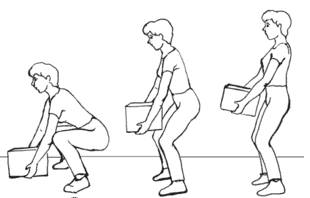
\includegraphics[width=60mm,scale=0.7]{./images/sollevamento_corretto.png} 
\makebox[\linewidth]{}
\captionof{figure}{Sollevamento corretto.}
\end{minipage}
\end{center}
\makebox[\linewidth]{}
\makebox[\linewidth]{}

\subsection{Movimento scorretto}
	Un modo scorretto di sollevare un carico è invece illustrato nella seguente figura, dove non si utilizzano le gambe, che rimangono stese durante tutta l'esecuzione della manovra, per aiutarsi nella distribuzione del peso, ma ci si piega con la sola schiena, esponendola di fatto a un alto rischio di disturbi dovuti a sovraccarico biomeccanico delle vertebre e dei dischi intervertebrali. Tale movimento è assolutamente da evitare. \\

\makebox[\linewidth]{}
\begin{center}
\begin{minipage}{0.48\linewidth}
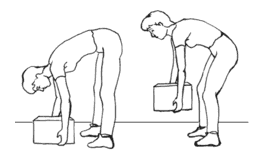
\includegraphics[width=60mm,scale=0.7]{./images/sollevamento_scorretto.png} 
\makebox[\linewidth]{}
\captionof{figure}{Sollevamento scorretto.}
\end{minipage}
\end{center}




	\clearpage

% ----- CAPITOLO III : raccolta dati -------
	\section{Raccolta dati}
Per poter eseguire uno studio del rischio che corre una persona, sollevando un carico elevato, si affronta una prima fase in cui si raccolgono i dati relativi alla movimentazione di quest'ultima. \\
Dunque si rende necessario uno strumento che permetta di raccogliere e catalogare informazioni, con cui poter ricostruire il movimento e, in uno step successivo, eseguire un' analisi per poter quantificare il rischio. \\



	\subsection{Sistema per la raccolta ed il salvataggio di dati}


Il sistema, di cui occore munirsi, dovrà contenere al suo interno sensori di vario genere, che gli permettano di registrare i movimenti e le variazioni delle condizioni ambientali esterne, a cui è sottoposto. \\
I sensori che prenderemo in considerazione, di cui l'hardware dovrà essere munito, sono i seguenti:
\begin{itemize}
\item \textbf{Accelerometro triassiale}, misura l’accelerazione che subisce il dispositivo sui tre assi cardinali.
\item \textbf{Giroscopio triassiale}, misura la velocità angolare del dispositivo attorno ai tre assi del sistema di riferimento.
\item \textbf{Magnetometro triassiale}, misura l’intensità del flusso del campo magnetico terrestre relativamente ai tre assi del sistema di riferimento. Tramite questo tipo di sensore possiamo ricavare informazioni sull’angolo che questo dispositivo forma con il campo magnetico terrestre.
\item \textbf{Barometro}, misura la pressione atmosferica alla quale il dispositivo è sottoposto; grazie alla elevata sensibilità di questo sensore è possibile individuare variazioni di pressione anche molto piccole, dell’ordine dei mbar.\\ \\
\end{itemize}

\begin{center}
\begin{minipage}{0.48\linewidth}
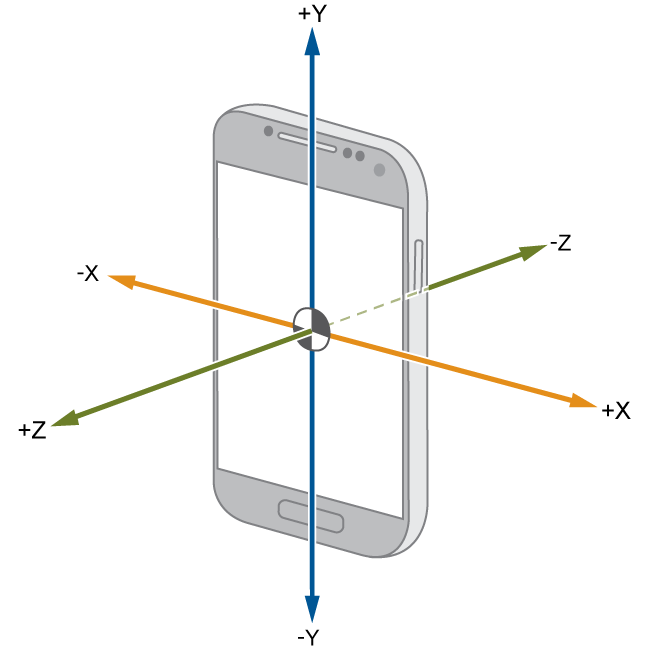
\includegraphics[width=70mm]{./images/triaxial_sensor.png}
\makebox[\linewidth]{}
\captionof{figure}{Sistema di coordinate (relativo allo smartphone) utilizzato dall'API Sensor.}
\end{minipage}
\end{center}


\makebox[\linewidth]{}
\makebox[\linewidth]{}
Un'altra proprietà che il nostro sistema deve possedere è essere \textbf{mini-invasivo}, infatti la persona che utilizza uno strumento di questo genere, non dovrebbe quasi accorgersi della sua presenza, affinché non si senta eccessivamente controllato oppure disturbato nei movimenti che compie; questo ci permetterà di effettuare delle misurazioni naturali e non falsate.


% ----- APPLICAZIONE ANDROID -----
	\subsection{Applicazione Android per la rccolta}
La soluzione che abbiamo trovato, che rispecchia i requisiti sopra riportati è un'applicazione Android, che gira su due dispositivi hardaware distinti: smartphone e smartwatch. \\ 
La scelta del sistema operativo, su cui si basa il sistema, è dovuta a vari fattori; in primo luogo la vasta gamma di prodotti, su cui è installato Android, molto differenti tra loro sia per caratteristiche, che per fasce di prezzi. Inoltre l'applicazione è stata sviluppata sull’IDE Android Studio, che integra interessanti funzionalità sia per la creazione di interfacce grafiche, sia per la parte relativa all’accesso al file system dei dispositivi compatibili. \\
In particolare durante lo svolgimento della tesi è stato adoperato uno smartphone Samsung Galaxy S6, sistema operativo Android 7.0 e uno smartwatch Huawei Watch 2, sistema operativo Wear OS 2.0 . \\
Di seguito i 3 moduli principali, nei quali è organizzato il progetto:
\begin{itemize}
\item mobile
\item wear
\item shared\_mobile\_watch \\
\end{itemize}
Il fine di questo sistema è produrre nel file system del telefono, in particolare nella directory "Documents", \textit{Environment.DIRECTORY\_DOCUMENTS}, otto file CSV: quattro relativi allo smartphone \textit{magnetometr\_phone, gyroscope\_phone, accelerometr\_phone, pressure\_phone} e quattro relativi allo smartwatch \textit{magnetometr\_watch, gyroscope\_watch, accelerometr\_watch, pressure\_watch}; ognuno di questi 4 file descrive il segnale proveniente da uno dei sensori precedentemente citati. \\


\makebox[\linewidth]{}
\begin{minipage}{\linewidth}
\begin{center}
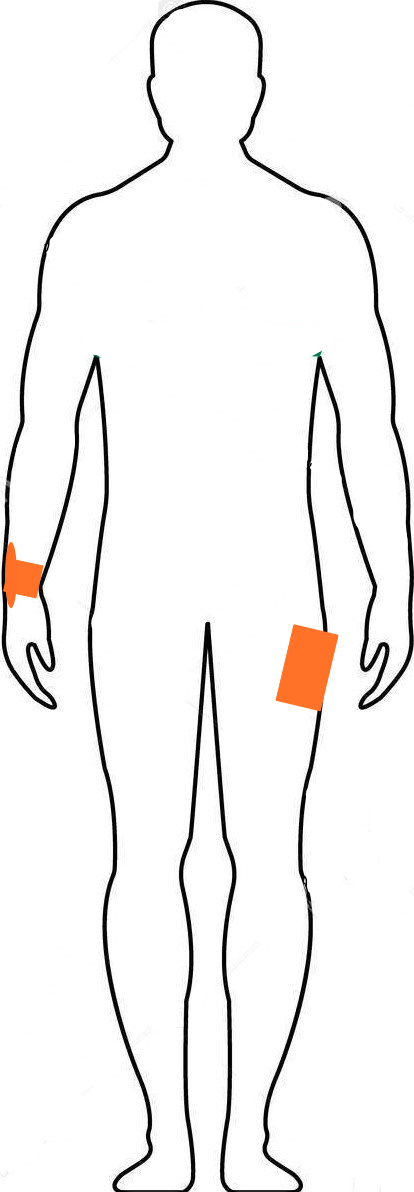
\includegraphics[width=35mm]{./images/sagoma_phone_watch.jpg} 
\makebox[\linewidth]{}
\captionof{figure}{Posizionamento dei dispositivi indossabili sull'utente.}
\end{center}
\end{minipage}
\makebox[\linewidth]{}
\makebox[\linewidth]{}


% ----- MODULO WEAR -----
\subsubsection{Modulo wear}
Il modulo wear implementa la parte dell’applicazione relativa allo smartwatch, essa ha le seguenti funzionalità: raccogliere i dati provenienti dai suoi sensori ed inviarli tramite bluetooth al telefono.\\
Di seguito non verrà riportato il codice di tutto il modulo, ma solamente la parte relativa alla raccolta dei dati e all’invio.
Nella seguente porzione di codice viene mostrato il callback che viene chiamato ogni volta che il valore di uno dei sensori subisce un cambiamento: ad ogni chiamata viene inserito nel buffer buffer (che può contenere 50 elementi) un oggetto che contiene informazioni relative al cambiamento appena avvenuto.
\makebox[\linewidth]{}
\makebox[\linewidth]{}

% ----- android wearable module -----
\begin{lstlisting}[language=Java,  basicstyle=\footnotesize]
public class MainActivity extends WearableActivity implements SensorEventListener {

    private TextView textView;
    private SensorManager sensorManager;
    ArrayList<Sensor> sensorList;
    DataSensor buffer[];
    int quanti;
    int iterazione = 0;
    ArrayList<Integer> type;
    boolean running;

    @Override
    protected void onCreate(Bundle savedInstanceState) {
        super.onCreate(savedInstanceState);
        setContentView(R.layout.activity_main);
        textView = findViewById(R.id.text);

        // register sensor
        sensorManager = (SensorManager) getSystemService(Context.SENSOR_SERVICE);
        sensorList = new ArrayList<Sensor>();
        sensorList.add(sensorManager.getDefaultSensor(Sensor.TYPE_MAGNETIC_FIELD));
        sensorList.add(sensorManager.getDefaultSensor(Sensor.TYPE_GYROSCOPE));
        sensorList.add(sensorManager.getDefaultSensor(Sensor.TYPE_ACCELEROMETER));
        sensorList.add(sensorManager.getDefaultSensor(Sensor.TYPE_PRESSURE));

        quanti = 0;
        buffer = new DataSensor[50];
        for(int i=0; i<50; i++)
            buffer[i] = new DataSensor();

        running = false;
        setAmbientEnabled();
    }

    public void startButton(View v) {
        if(!running) {
            Log.i("start", "start");
            Toast.makeText(getBaseContext(), "Start recording...", Toast.LENGTH_LONG).show();
            for (Sensor s: sensorList) {
                sensorManager.registerListener(this, s, SensorManager.SENSOR_DELAY_FASTEST);
            }
            running = true;
        }
    }

    public void stopButton(View v)
    {
        if(running) {
            Log.i("stop", "stop");
            Toast.makeText(getBaseContext(), "Stop recording...", Toast.LENGTH_LONG).show();
            sensorManager.unregisterListener(this);
            running = false;
        }
    }

    public void onSensorChanged(SensorEvent event) {

        buffer[quanti].setSensorType(event.sensor.getType());
        buffer[quanti].setTimestamp(String.valueOf(event.timestamp));
        buffer[quanti].setValue0(String.valueOf(event.values[0]));
        if(event.sensor.getType() != Sensor.TYPE_PRESSURE){
            buffer[quanti].setValue1(String.valueOf(event.values[1]));
            buffer[quanti].setValue2(String.valueOf(event.values[2]));
        }

        quanti++;

        if (quanti == 50) {
            new SendMessage("/data", buffer).start();
            for(int i=0; i<50; i++){
                Log.i("data" + iterazione + " " + i, buffer[i].getSensorType()+" ");
            }
            quanti = 0;
            iterazione++;
        }
    }

    public void onAccuracyChanged(Sensor sensor, int accuracy) {}

    class SendMessage extends Thread {
        String path;
        DataSensor message[];

        //Constructor for sending information to the Data Layer//
        SendMessage(String p, DataSensor m[]) {
            path = p;
            message = m;
        }

        public void run() {

            //Retrieve the connected devices//
            Task<List<Node>> nodeListTask =
                    Wearable.getNodeClient(getApplicationContext()).getConnectedNodes();
            try {

                //Block on a task and get the result synchronously//
                List<Node> nodes = Tasks.await(nodeListTask);
                for (Node node : nodes) {
                    try {
                        ByteArrayOutputStream bos = new ByteArrayOutputStream();
                        ObjectOutputStream oos = new ObjectOutputStream(bos);
                        oos.writeObject(message);

                        //Send the message//
                        Wearable.getMessageClient(MainActivity.this).sendMessage(node.getId(),
								 path, bos.toByteArray());
                        oos.close();
                        bos.close();
                    }
                    catch(IOException e){e.printStackTrace();}
                }
            }
            catch (ExecutionException e) {e.printStackTrace();}
            catch (InterruptedException e) {e.printStackTrace();}
        }
    }
}
\end{lstlisting}


% ----- MODULO SHARED -----
\subsubsection{Mosulo shared\_mobile\_watch}
Questo modulo molto semplice è una libreria android richiamata dai moduli mobile e wear e contenente un’unica classe DataSensor che implementa l’interfaccia Serializable, poichè le istanze di tale classe dovranno essere inviate dall’orologio al telefono. 
Tale classe memorizza le informazioni principali relative ad un cambiamento di valore di un sensore:  il tipo di sensore sensorType, tre valori value0, value1, value2 e l’istante in cui è avvenuto il cambiamento timestamp.
E’ buona pratica aggiungere in tutti i progetti, che contengono più moduli che lavorano con gli stessi tipi di classi, una libreria android, che contenga le classi necessarie ad entrambi; nonostante questo possa creare alcuni problemi durante la compilazione se ci sono aggiornamenti della versione.
\makebox[\linewidth]{}
% ----- android shared module -----
\begin{lstlisting}[language=Java,  basicstyle=\footnotesize]
public class DataSensor implements Serializable {
    private int sensorType;
    private String value0;
    private String value1;
    private String value2;
    private String timestamp;

    public int getSensorType() {
        return sensorType; }
    public void setSensorType(int sensorType) {
        this.sensorType = sensorType; }

    public String getValue0() {
        return value0; }
    public void setValue0(String value0) {
        this.value0 = value0; }

    public String getValue1() {
        return value1; }
    public void setValue1(String value1) {
        this.value1 = value1; }

    public String getValue2() {
        return value2; }
    public void setValue2(String value2) {
        this.value2 = value2; }

    public String getTimestamp() {
        return timestamp; }
    public void setTimestamp(String timestamp) {
        this.timestamp = timestamp; }

    public byte[] getBytes() {
        ByteArrayOutputStream bos = new ByteArrayOutputStream();
        ObjectOutput out = null;
        try {
            out = new ObjectOutputStream(bos);
            out.writeObject(this);
            out.flush();
            return bos.toByteArray();
        } catch (IOException e) {
            Log.e("DataSensor", e.getLocalizedMessage(), e);
        } finally {
            try {
                bos.close();
            } catch (IOException ex) {
                // ignore close exception
            }
        }
        return new byte[]{};
    }
}
\end{lstlisting}


% ----- MODULO MOBILE -----
\subsubsection{Modulo mobile}
In questo modulo vengono ricevuti i dati provenienti dall’orologio grazie al service MessageService, dichiarato nel manifesto.\\
\makebox[\linewidth]{}
% ----- android mobile module -----
\begin{lstlisting}[language=Java,  basicstyle=\footnotesize]
public class MessageService extends WearableListenerService {

    public void onMessageReceived(MessageEvent messageEvent) {

        if (messageEvent.getPath().equals("/data")) {
            final DataSensor[] message = getDataSensor(messageEvent.getData());
            Intent messageIntent = new Intent();
            messageIntent.setAction(Intent.ACTION_SEND);
            messageIntent.putExtra("message", message);
            LocalBroadcastManager.getInstance(this).sendBroadcast(messageIntent); }
    }

    public DataSensor[] getDataSensor(byte[] b) {
        ByteArrayInputStream bis = new ByteArrayInputStream(b);
        ObjectInput in = null;
        try {
            in = new ObjectInputStream(bis);
            return (DataSensor[]) in.readObject();
        }
        catch (IOException e) { Log.e("MainMobile", e.getLocalizedMessage(), e);}
        catch (ClassNotFoundException e) { Log.e("MainMobile", e.getLocalizedMessage(), e); }
        finally {
            try {
                if (in != null) {
                    in.close();
                }  } catch (IOException ex) {ex.printStackTrace();} }
        return null; }
}
\end{lstlisting}
\makebox[\linewidth]{}
Tale classe, non scrive direttamente i dati sul file, ma li invia in broadcast ad altri thread. Tali dati vengono ricevuti e scritti da un un thread Receiver, dichiarato nel metodo onCreate e richiamato all’avvio dell’applicazione. Ogni volta che viene inviato un buffer di 50 elementi dal service precedentemente descritto, viene invocato questo metodo del thread che riceve il pacchetto e ne trascrive i dati contenuti, chiamando la funzione writeFile(DataSensor buf[]), di cui non è riportato il codice, in quanto molto semplice (chiama la open su un file, scrive su di esso con il metodo write ed infine chiude il file con il metodo close). 

\makebox[\linewidth]{}
 % ----- android mobile module -----
\begin{lstlisting}[language=Java,  basicstyle=\footnotesize]
public void onReceive(Context context, Intent intent) {
        // ottengo un array di oggetti DataSensor da uno stream di byte
        DataSensor buffer[];
        buffer = (DataSensor[]) intent.getSerializableExtra("message");

        for(int i=0; i<50; i++){
            Log.i("data" + iterazione + " " + i, buffer[i].getSensorType() + " " );
        }
        iterazione++;
        writeFile(buffer);
    }
\end{lstlisting}
\makebox[\linewidth]{}
Sempre in questo modulo, inoltre, viene fatta la registrazione dei sensori contenuti nel telefono, similmente a come viene fatta nel modulo wear. Per evitare ripetizioni del codice nella documentazione, è omessa anche questa parte.

\makebox[\linewidth]{}


% ----- CAPITOLO SUGLI ESPERIMENTI -----
	\subsection{Esperimenti di registrazione}
Dopo essersi muniti di uno strumento che rispecchi i requisiti precedentemente elencati, si  affronta una fase in cui si eseguono uno o più esperimenti di registrazione: ogni esperimento è definito da un set di azioni, che dovranno essere svolte da un candidato, mentre il sistema di registrazione e salvataggio dei dati memorizza tutte le informazioni neccessarie a ricostruire la movimentazione compiuta.

% ----- ESPERIMENTO I -----
	\subsubsection{Esperimento 1}
L' esperimento svolto è piuttosto semplice, vengono eseguite essenzialmente 3 azioni in loop:
\begin {itemize}
\item camminata
\item sollevamento del carico 
\item rilascio del carico.
\end{itemize}
La ultime due azioni possono essere fatte in maniera sicura oppure dannosa per la schiena. \\
Di seguito è riportato uno schema del modulo:\\

\makebox[\linewidth]{}
\begin{minipage}{\linewidth}
\begin{center}
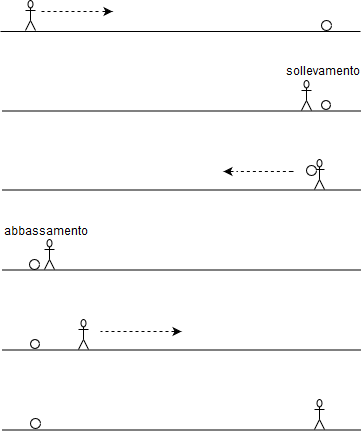
\includegraphics[width=60mm,scale=0.7]{./images/esperimento1.png} 
\makebox[\linewidth]{}
\captionof{figure}{Schema dei task dell'esperimento 1.\\}
\end{center}
\end{minipage}
\makebox[\linewidth]{} 
\makebox[\linewidth]{}
\makebox[\linewidth]{}
\makebox[\linewidth]{}
Questo schema riassume un ciclo del percorso totale. L’esperimento completo prevederà 2 cicli, per un totale di 2 sollevamenti e due rilasci del carico\\ \\
In generale gli esperimenti da svolgere, dovrebbero essere molteplici e dovrebbero prevedere una gamma molto più ampia di azioni, che un lavoratore potrebbe compiere: permanenza alla scrivania, utilizzo di dispositivi elettronici, utilizzo di attrezzatura da operaio. Inoltre dovrebbero essere effettuati in condizioni ambientali differenti, per poter realizzare un sistema il più universale possibile.

\clearpage


% ------ CAPITOLO IV : analisi ------
\section{Analisi}
La fase che segue la raccolta è l'analisi dei dati ottenuti dall'esperimento eseguito. Questo passaggio prevede l'importazione dei dati sull'ambiente di calcolo MATLAB, l'analisi e la processazione dei segnali, mediante l'utilizzo  del pacchetto Signal Processing Toolbox 8.1. \\
Questa fase di analisi si divide in due sottofasi:
\begin {itemize}
\item Individuazione dell'istante in cui avviene il task del sollevamento. L'obiettivo di questa prima fase dell'analisi è individuare gli istanti, in cui viene eseguito il movimento, in modo da non dover passare  passare alla fase della classificazione tutti i segnali dei sensori, ma solamente alcune porzioni, e rendere il sistema più efficiente.
\item Classificazione della manovra. Questa fase viene fatta da una rete neurale, che riceve in input i parametri più significativi, calcolati dalle porzioni di segnale individuate nella fase di detection, e classifica la manovra come \textit{corretta}, \textit{scorretta} o \textit{carico assente}.
\end{itemize}

% ----- VISUALIZZAZIONE GRAFICI -----
\subsection{Visualizzazione grafici}
La prima fase di analisi ha previsto la creazione dei grafici, risultanti dalle rilevazioni degli otto sensori (relativi alla stessa registrazione), per poter eseguire avere una panoramica sull'andamento dei segnali collezionati, poter compiere le prime considerazioni ed inquadrare eventuali problemi che potrebbero insorgere.\\
Matlab mette a disposizione la funzione \textit{plot} per poter visualizzare grafici di forme diverse, in relazione ai tipi che vengono passati come argomento, quando la fuzione viene chiamata:  Se y `e un vettore, \textit{plot(x)} produce un grafico lineare degli elementi di y contro l’indice degli elementi di y.  Se venogno specificati due vettori come argomento,\textit{ plot(x, y) } produce un grafico, in cui i valori della x vengono posizionati sull'ascissa e quelli di y sull'ordinata. \\
 % si nota che sono grafici molto diversi perchè prodotti da segnali che hanno differenti caratteristiche.. signal preprocessing (o forse lo dico dopo?)

% ---- GRAFICI GIROSCOPIO ------
\subsubsection{Giroscopio smartphone}
\begin{minipage}{\linewidth}
\begin{center}
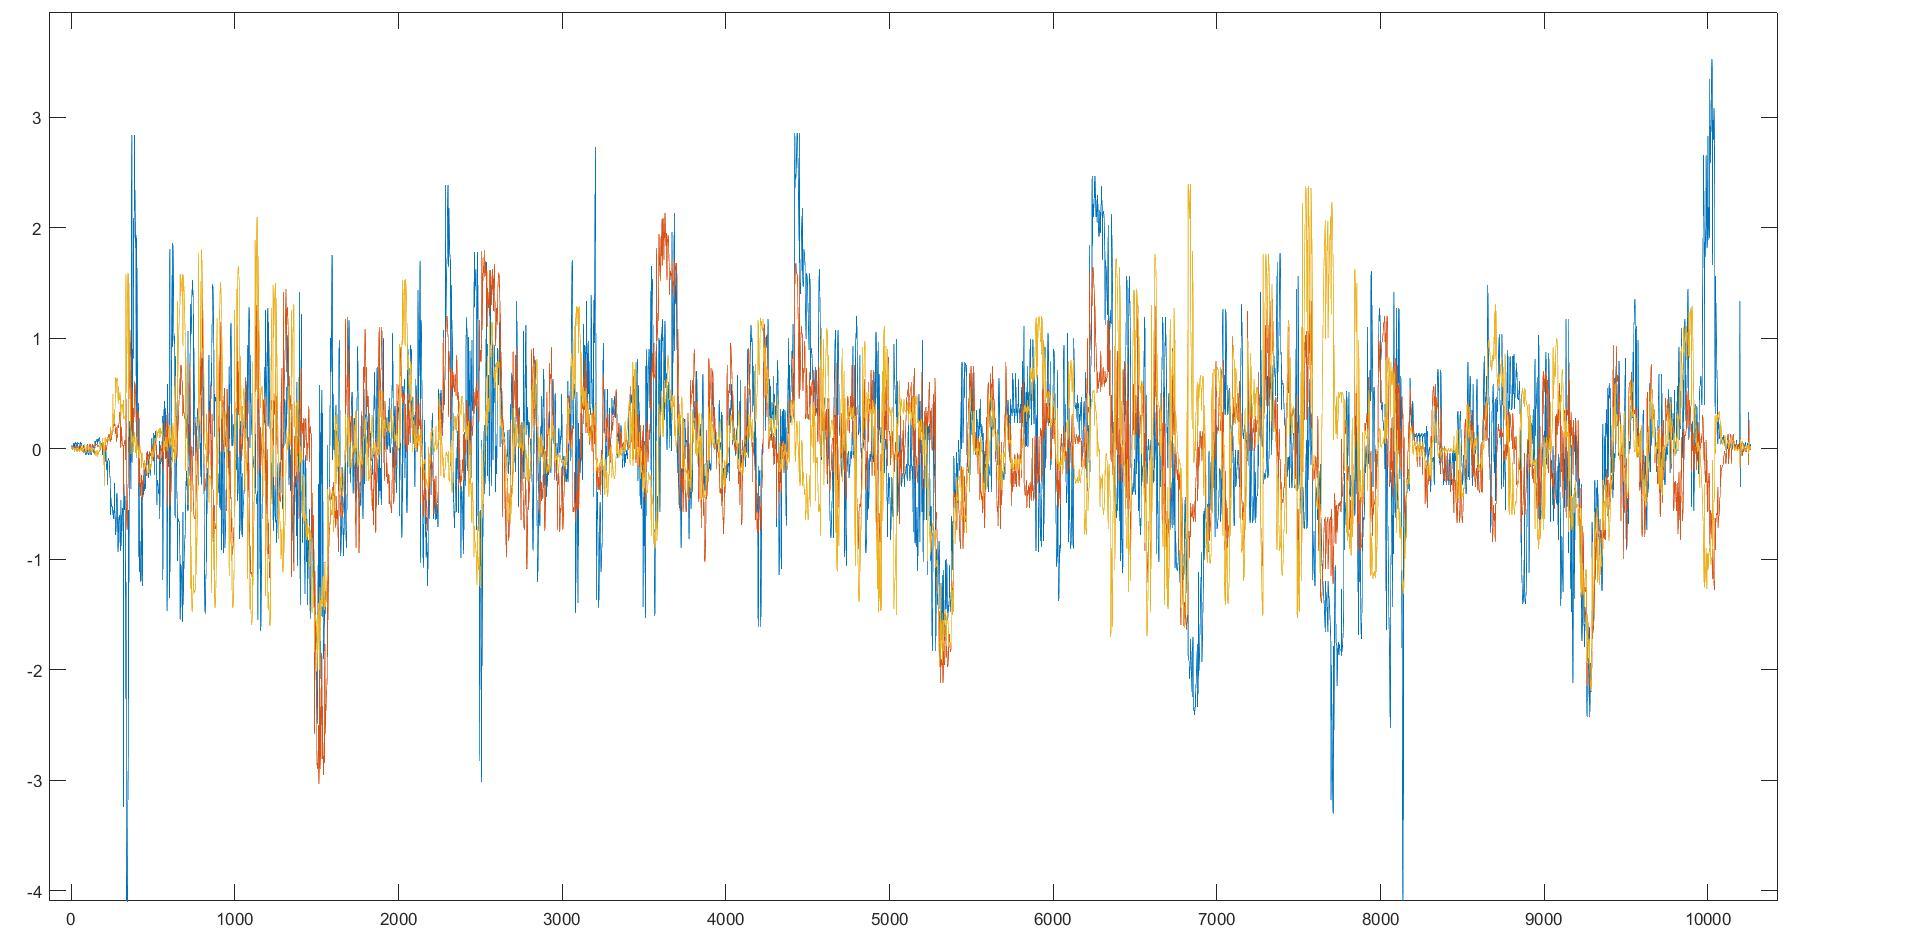
\includegraphics[width=160mm, height= 70mm]{./images/registrazione_tesi/gyrXYZ.jpg} 
\captionof{figure}{Grafico accelerometro triassiale dello smartphone.\\}
\end{center}
\end{minipage}
\makebox[\linewidth]{}
\makebox[\linewidth]{}\makebox[\linewidth]{}\makebox[\linewidth]{}
\makebox[\linewidth]{}\makebox[\linewidth]{}\makebox[\linewidth]{}
\makebox[\linewidth]{}\makebox[\linewidth]{}\makebox[\linewidth]{}

\clearpage

% ---- GRAFICI BAROMETRO ------
\subsubsection{Barometro smatwatch\\} 
\begin{minipage}{\linewidth}
\begin{center}
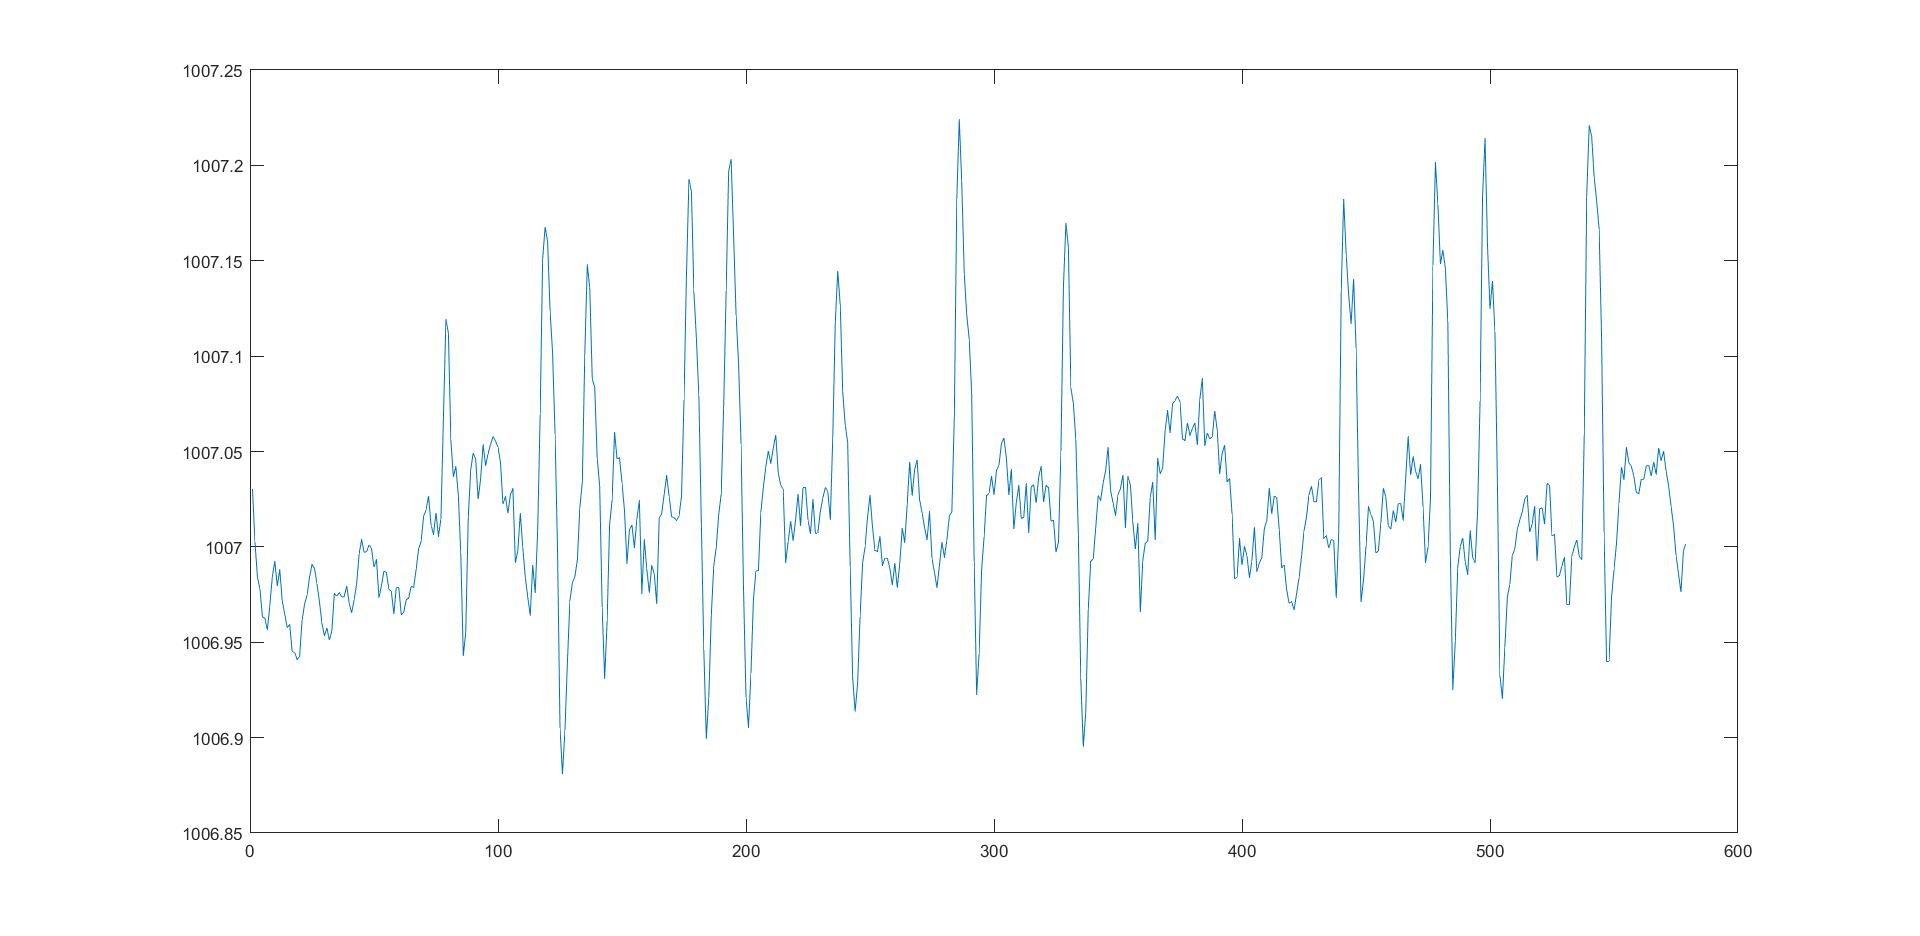
\includegraphics[width=160mm, height= 80mm]{./images/registrazione_tesi/pressure_phone.jpg} 
\captionof{figure}{Segnale barometrico dello smartphone.\\}
\end{center}
\end{minipage}
\makebox[\linewidth]{}
\makebox[\linewidth]{}\makebox[\linewidth]{}\makebox[\linewidth]{}
\makebox[\linewidth]{}\makebox[\linewidth]{}\makebox[\linewidth]{}
\makebox[\linewidth]{}\makebox[\linewidth]{}\makebox[\linewidth]{}
\makebox[\linewidth]{}\makebox[\linewidth]{}\makebox[\linewidth]{}

\subsubsection{Barometro smatphone\\} 
\makebox[\linewidth]{}
\begin{minipage}{\linewidth}
\begin{center}
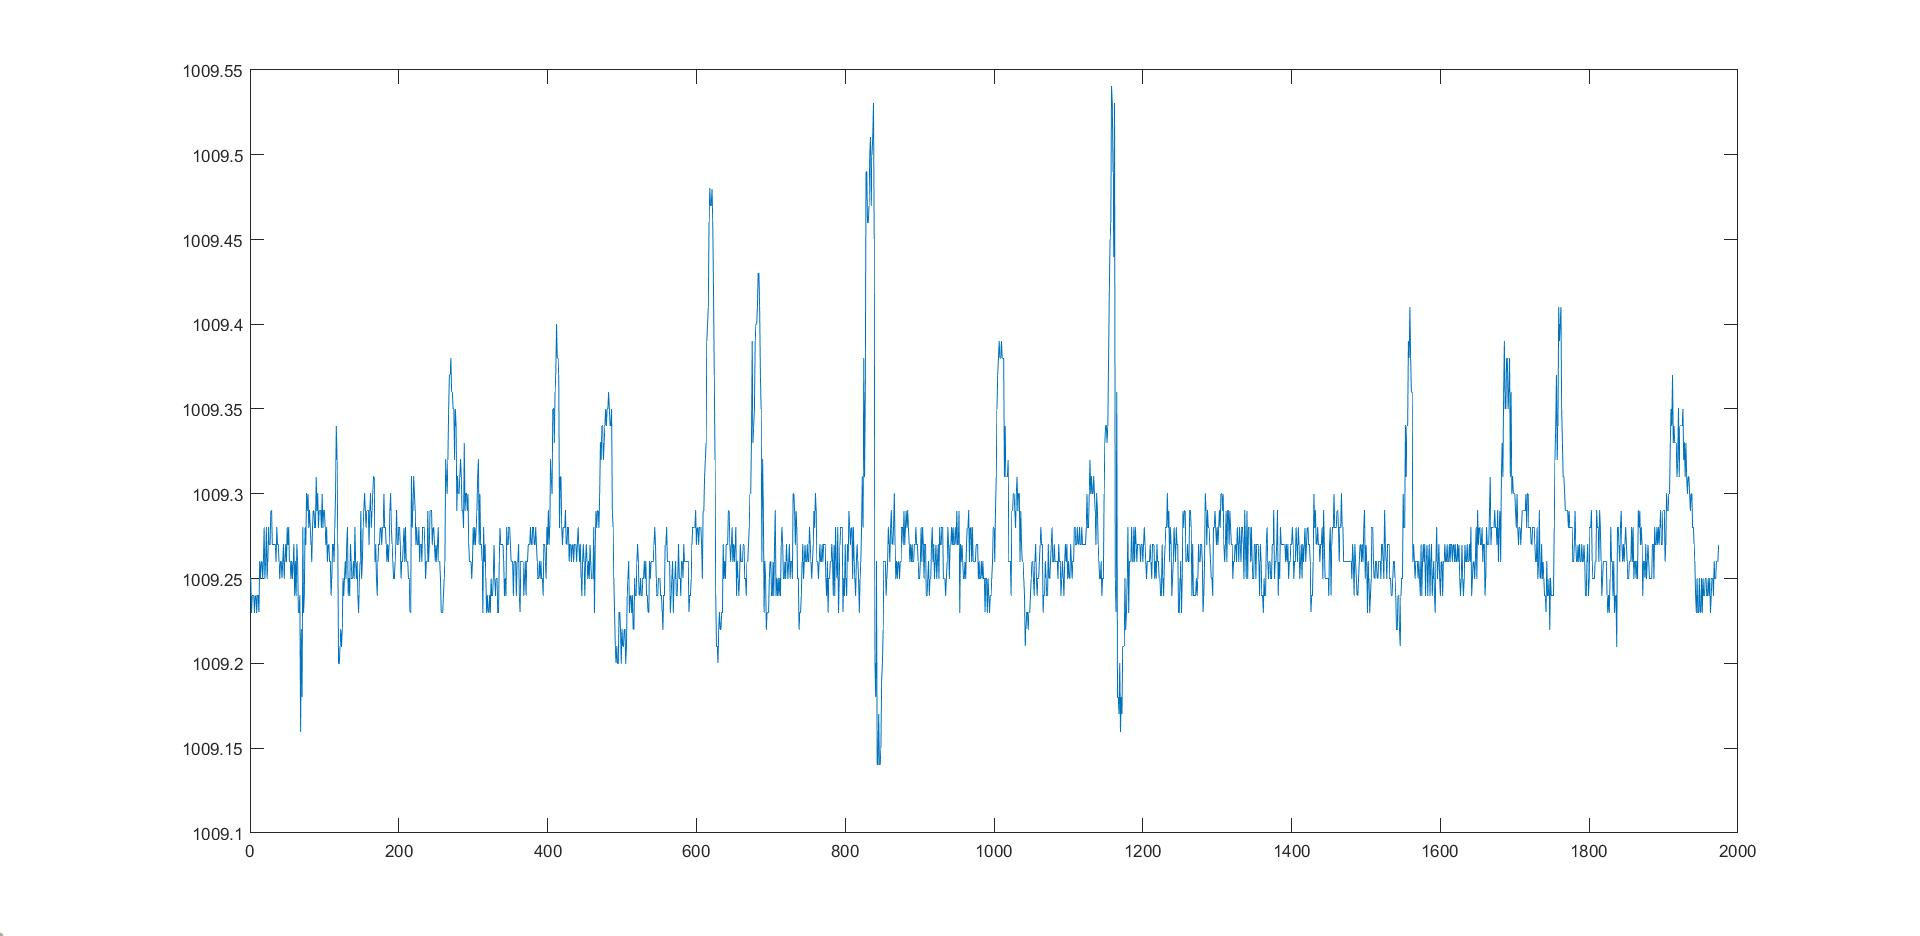
\includegraphics[width=160mm, height= 80mm]{./images/registrazione_tesi/pressure_watch.jpg} 
\captionof{figure}{Segnale barometrico dello smartphone.\\}
\end{center}
\end{minipage}

\clearpage

% ---- GRAFICI ACCELEROMETRO OROLOGIO ------
\subsubsection{Accelerometro smartwatch}
\begin{minipage}{\linewidth}
\begin{center}
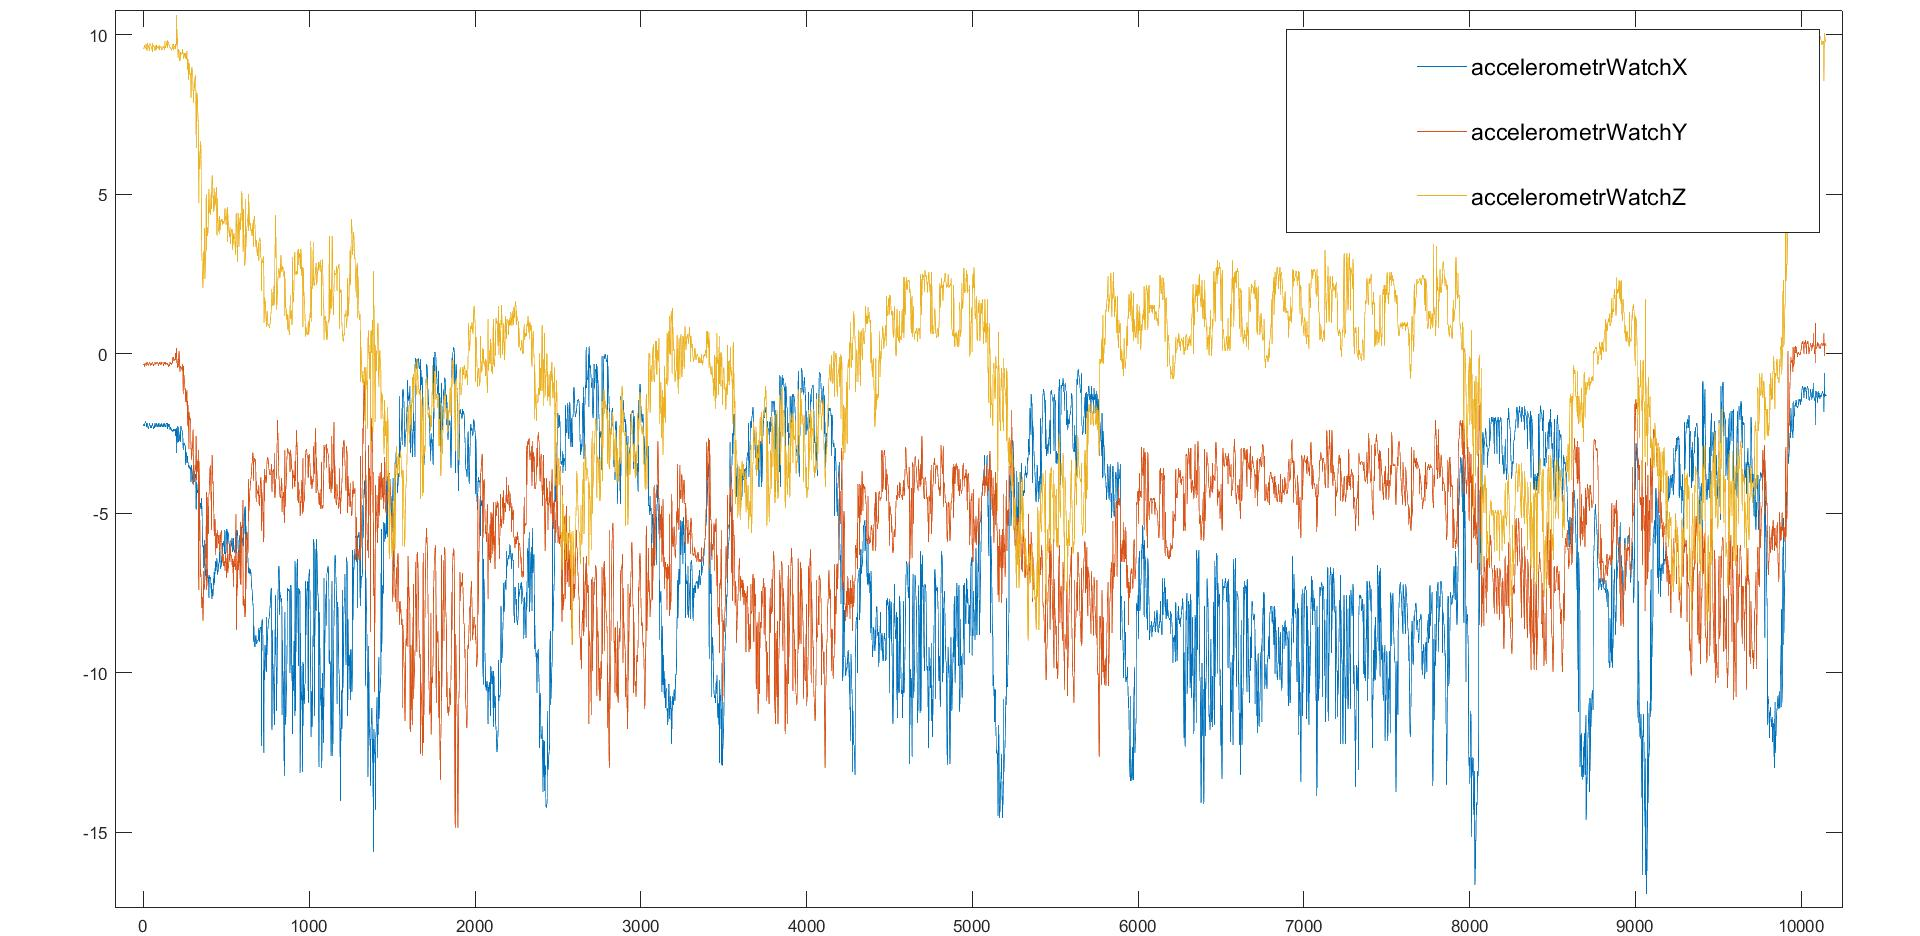
\includegraphics[width=160mm, height= 70mm]{./images/registrazione_tesi/accelerometrXYZ.jpg} 
\captionof{figure}{Grafico accelerometro triassiale dello smartwatch.\\}
\end{center}
\end{minipage}
\makebox[\linewidth]{}
\makebox[\linewidth]{}\makebox[\linewidth]{}\makebox[\linewidth]{}
\makebox[\linewidth]{}\makebox[\linewidth]{}\makebox[\linewidth]{}
\makebox[\linewidth]{}\makebox[\linewidth]{}\makebox[\linewidth]{}

% ---- X -----
\begin{minipage}{\linewidth}
\begin{center}
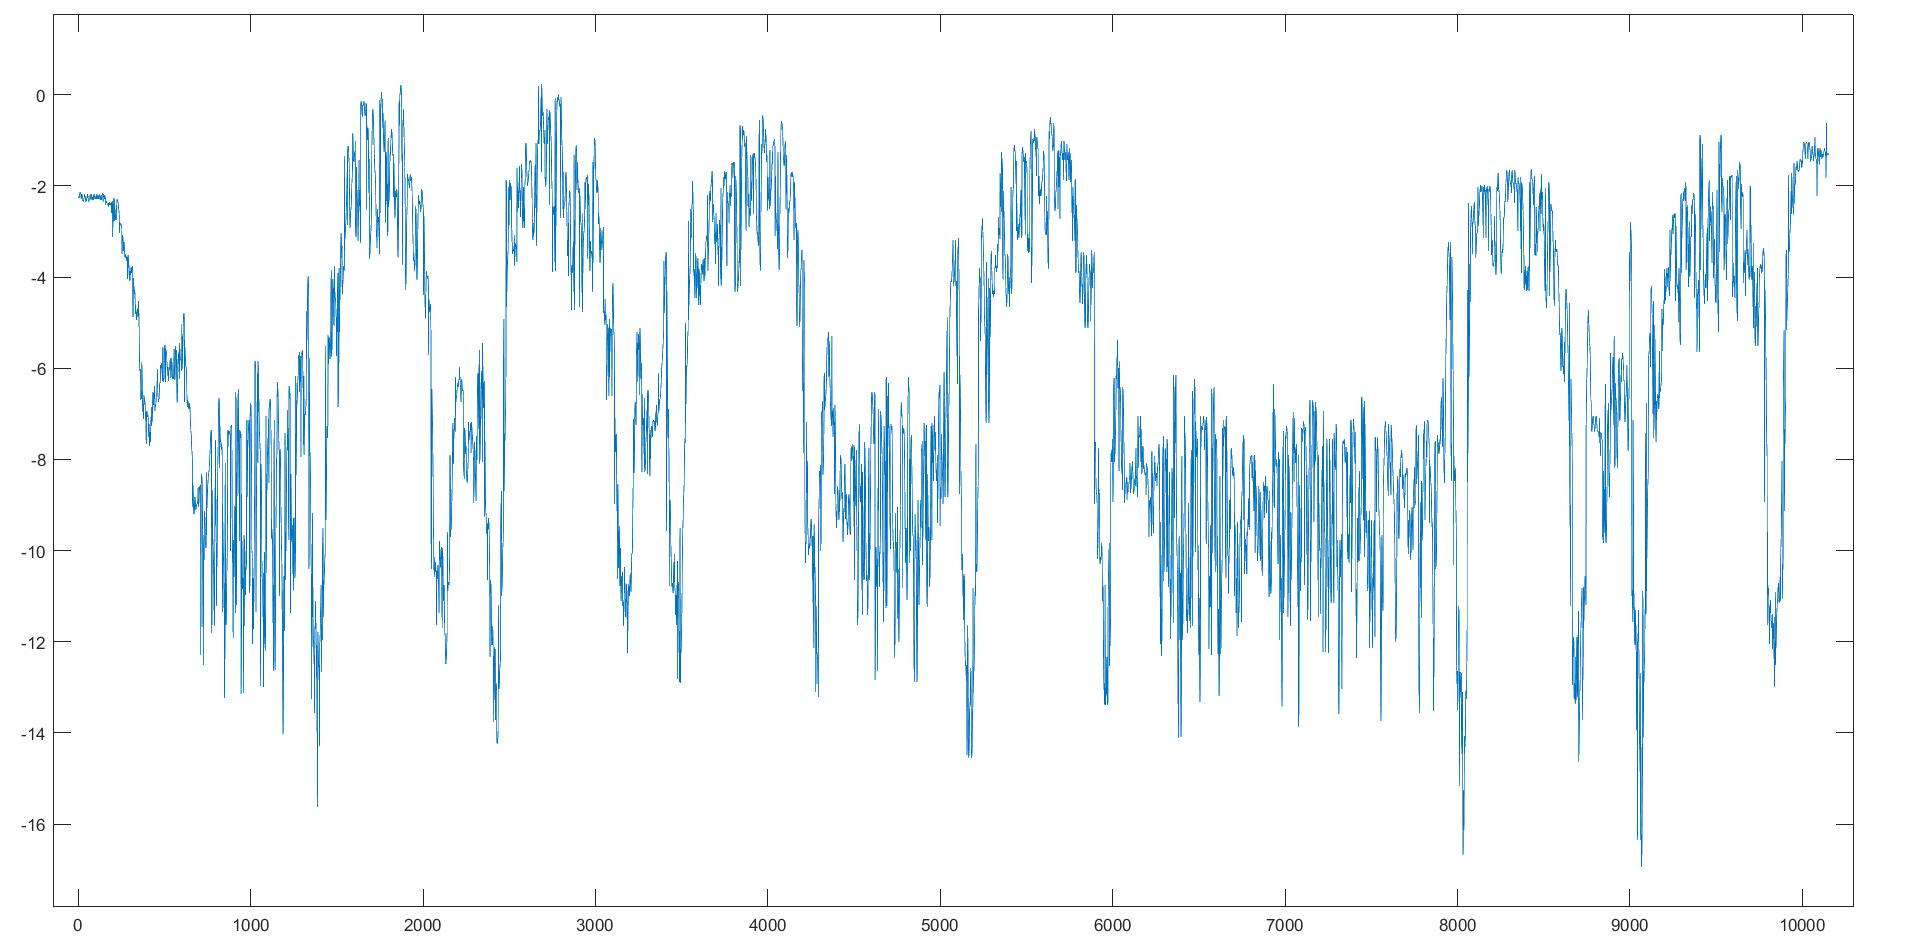
\includegraphics[width=154mm, height= 40mm]{./images/registrazione_tesi/accX.jpg} 
\end{center}
\end{minipage}
\makebox[\linewidth]{}

% ---- Y -----
\begin{minipage}{\linewidth}
\begin{center}
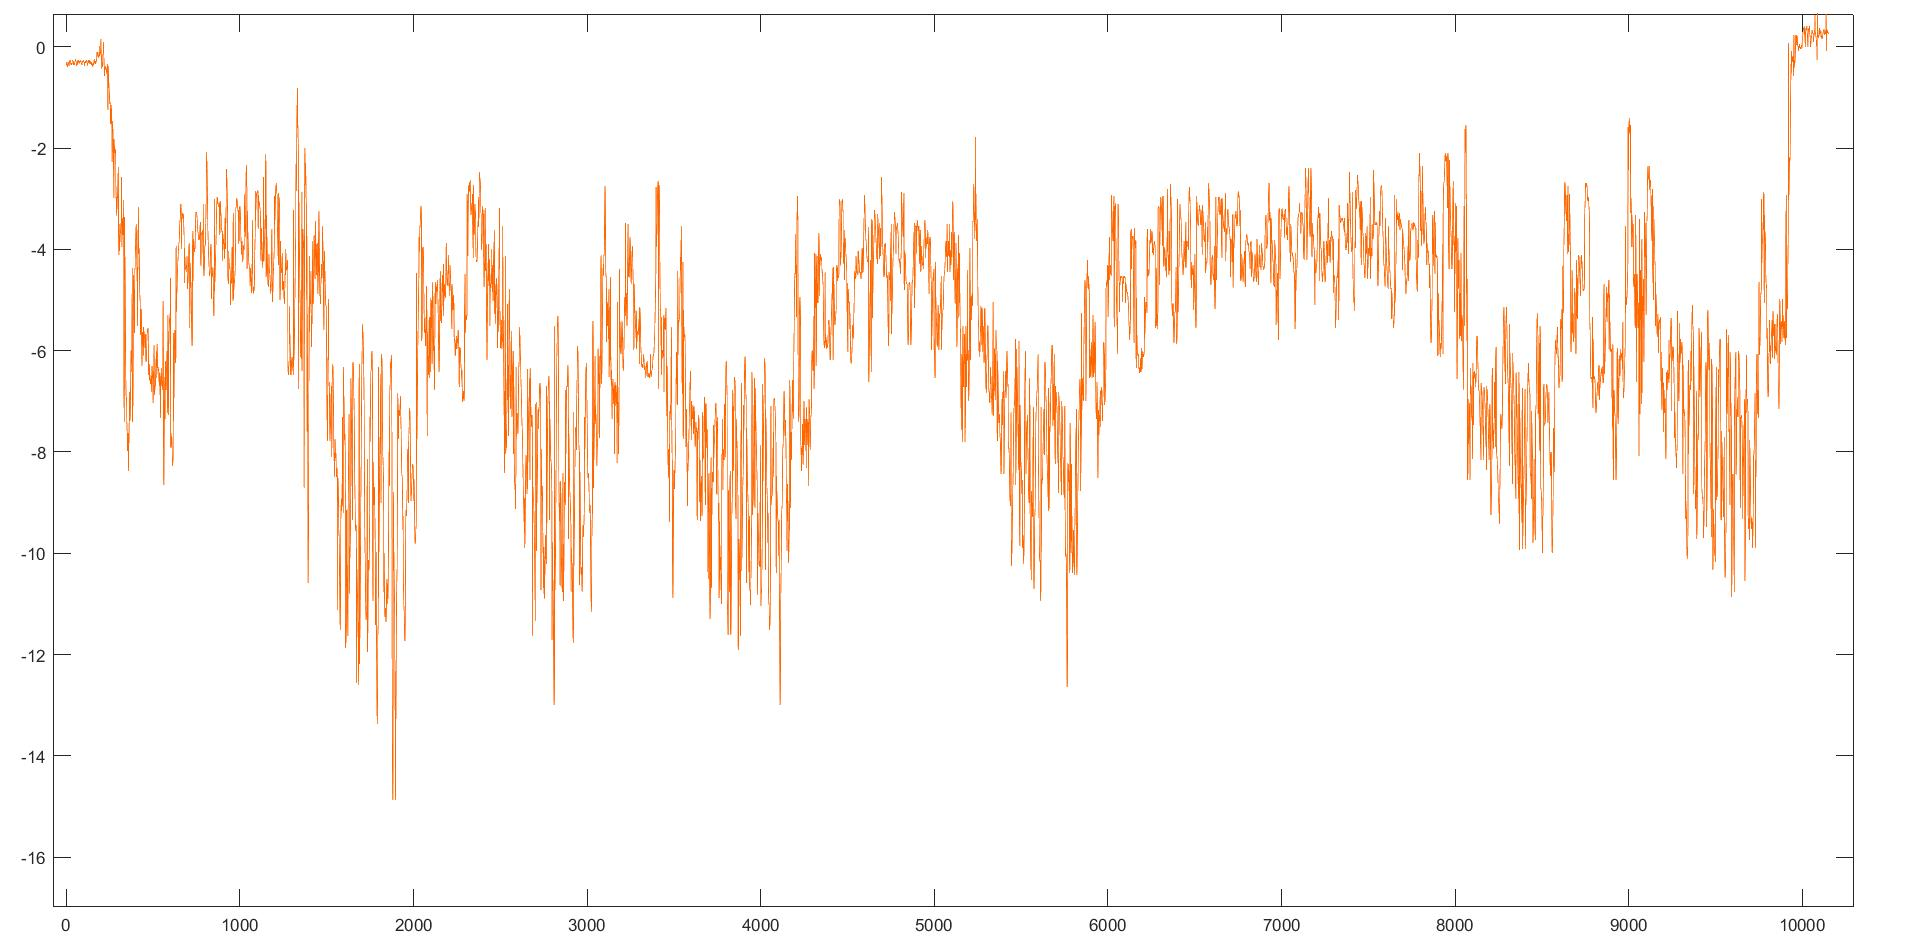
\includegraphics[width=154mm, height= 40mm]{./images/registrazione_tesi/accY.jpg} 
\end{center}
\end{minipage}
\makebox[\linewidth]{}

% ---- z -----
\begin{minipage}{\linewidth}
\begin{center}
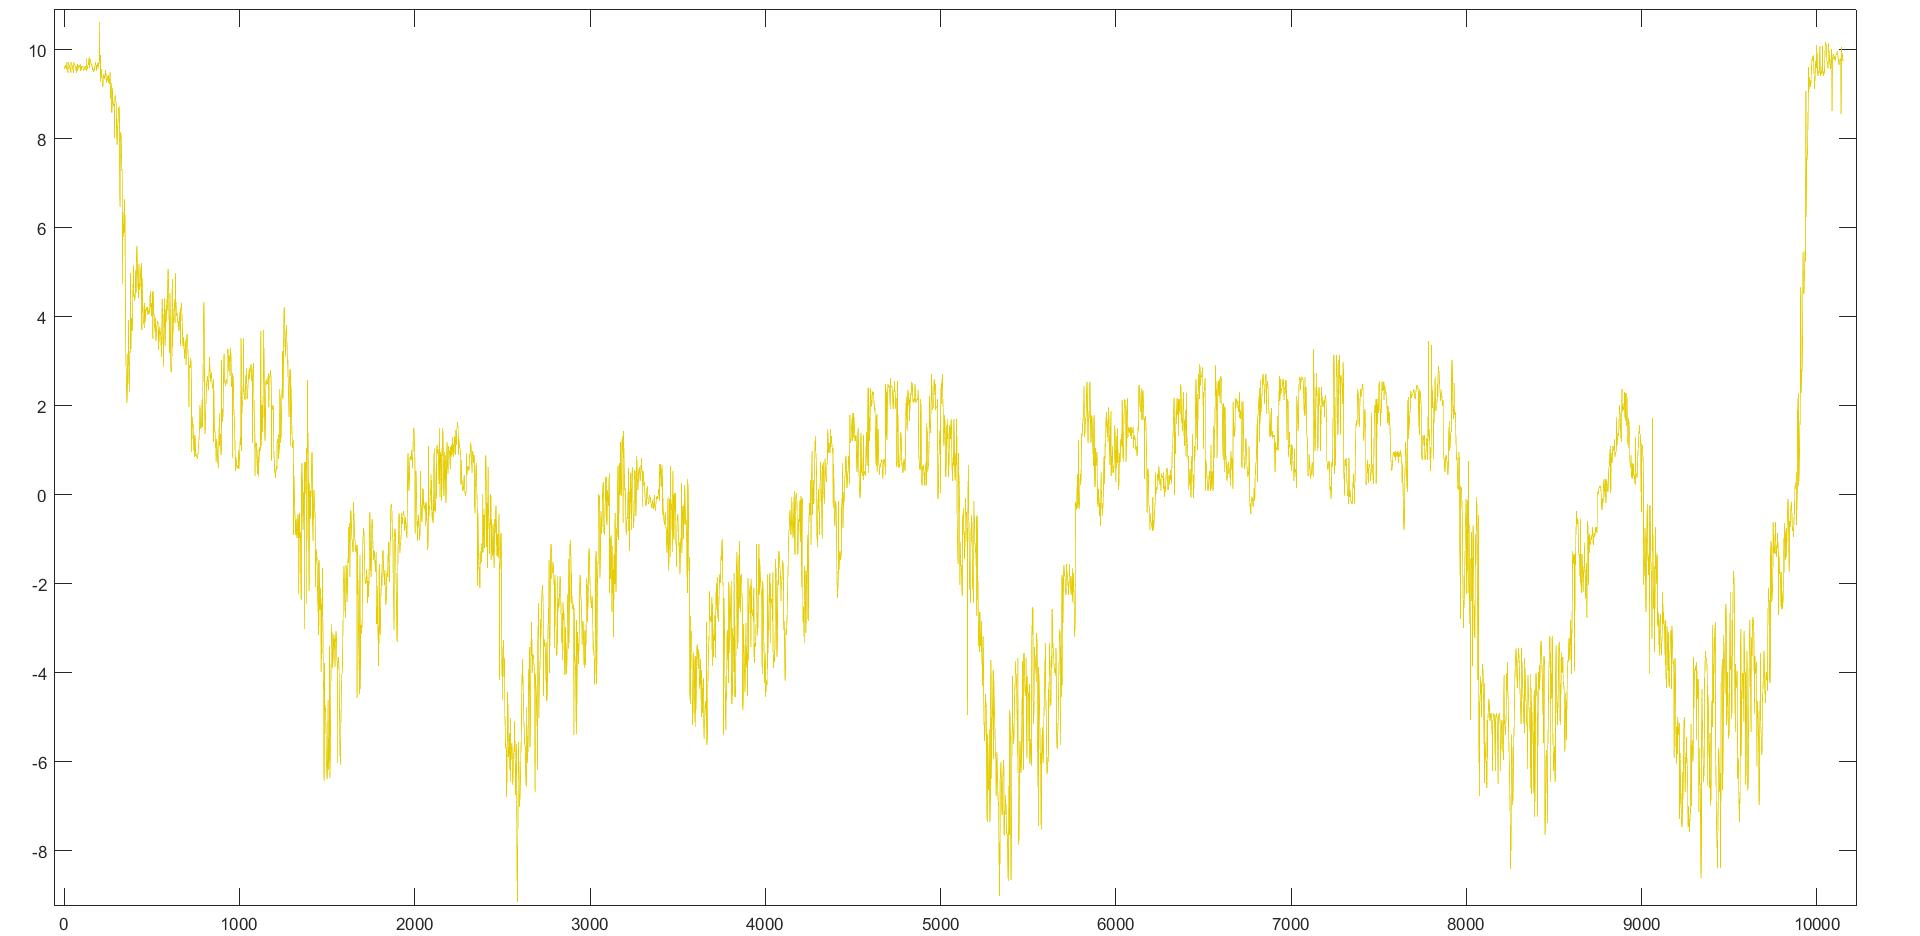
\includegraphics[width=154mm, height= 40mm]{./images/registrazione_tesi/accZ.jpg} 
\captionof{figure}{Scomposizione del segnale accelerometrico triassiale in tre grafici.\\}
\end{center}
\end{minipage}
\makebox[\linewidth]{}
\makebox[\linewidth]{}\makebox[\linewidth]{}\makebox[\linewidth]{}
\makebox[\linewidth]{}\makebox[\linewidth]{}\makebox[\linewidth]{}

% ---- GRAFICI ACCELEROMETRO TELEFONO------
\subsubsection{Accelerometro smartphone}
\begin{minipage}{\linewidth}
\begin{center}
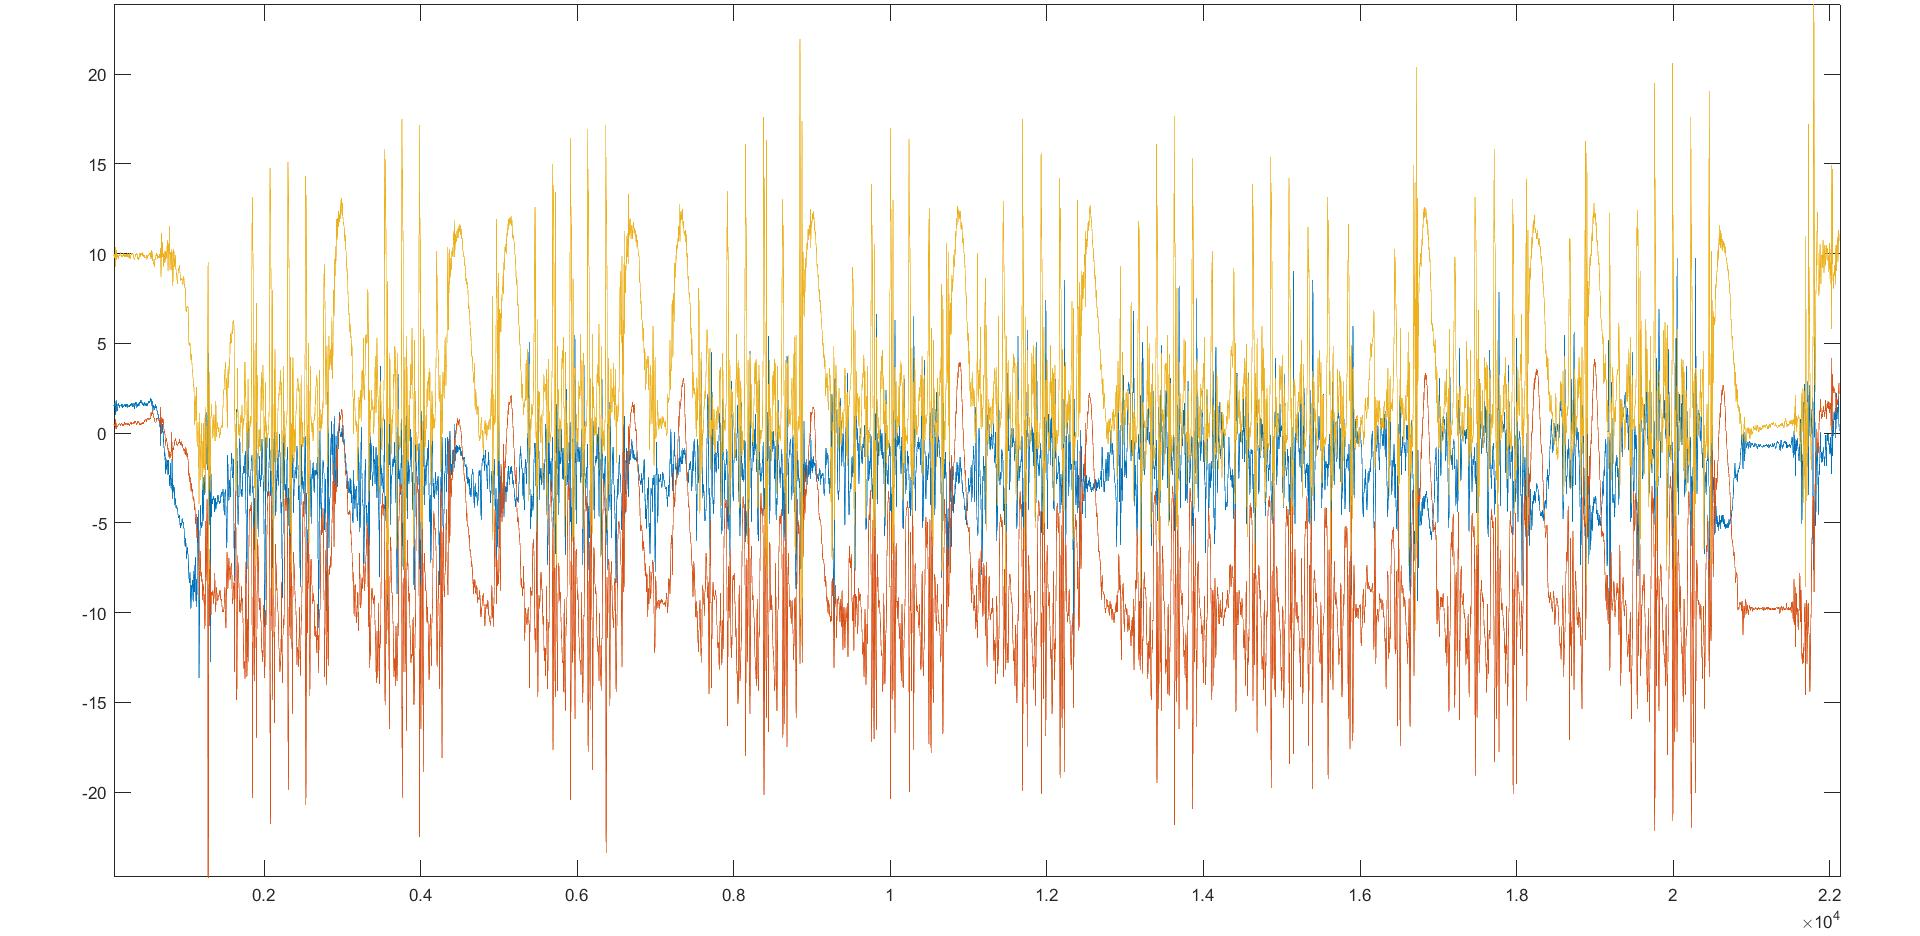
\includegraphics[width=160mm, height= 70mm]{./images/registrazione_tesi/acc_ph.jpg} 
\captionof{figure}{Grafico accelerometro triassiale dello smartphone.\\}
\end{center}
\end{minipage}
\makebox[\linewidth]{}
\makebox[\linewidth]{}\makebox[\linewidth]{}\makebox[\linewidth]{}
\makebox[\linewidth]{}\makebox[\linewidth]{}\makebox[\linewidth]{}
\makebox[\linewidth]{}\makebox[\linewidth]{}\makebox[\linewidth]{}

% ---- X -----
\begin{minipage}{\linewidth}
\begin{center}
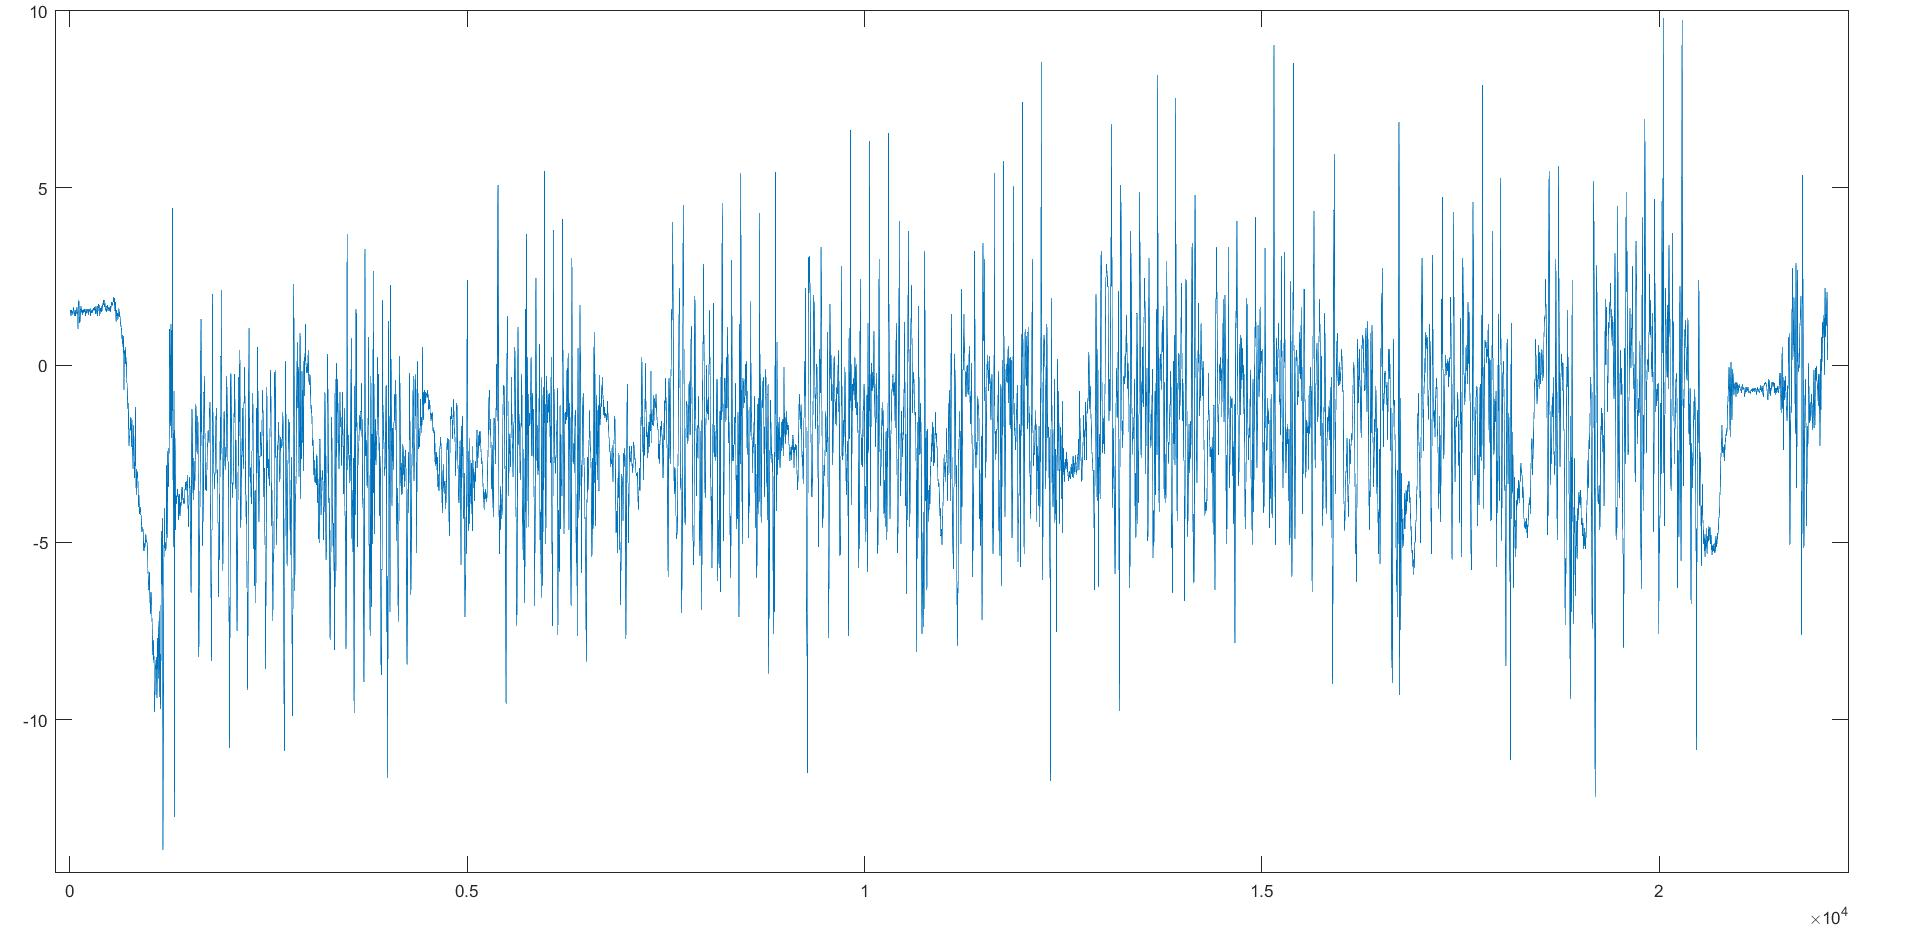
\includegraphics[width=154mm, height= 40mm]{./images/registrazione_tesi/acc_phX.jpg} 
\end{center}
\end{minipage}
\makebox[\linewidth]{}

% ---- Y -----
\begin{minipage}{\linewidth}
\begin{center}
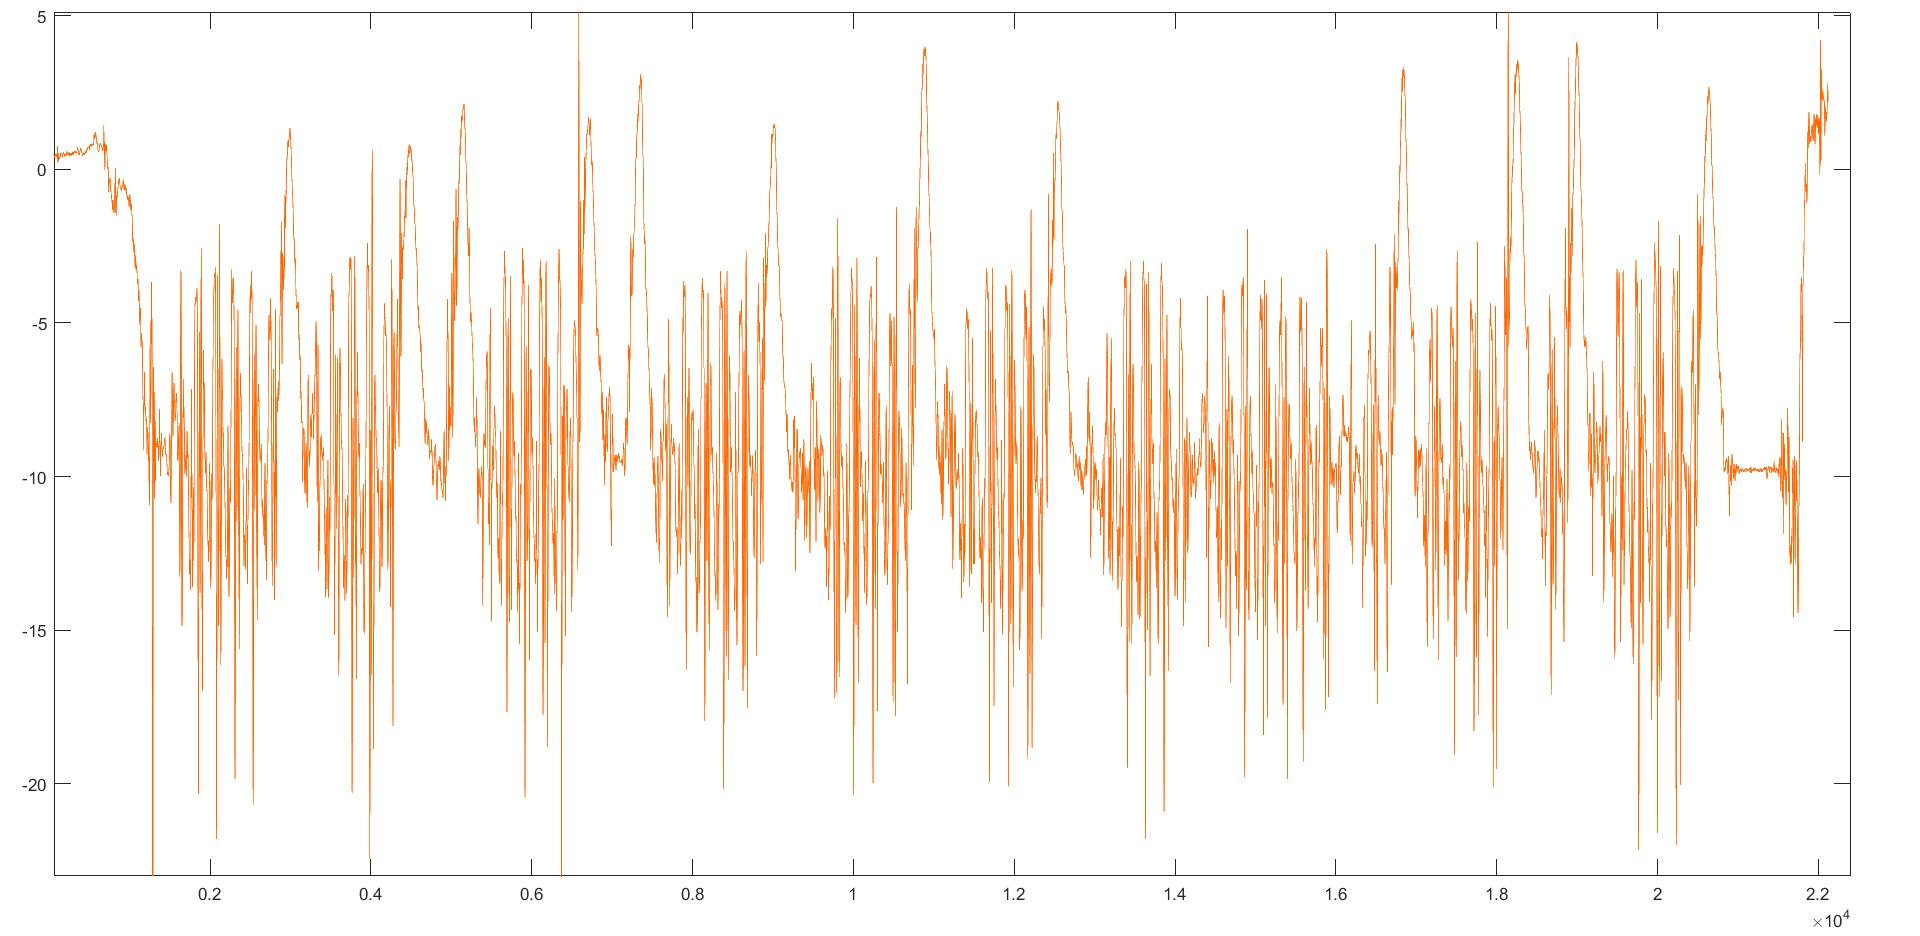
\includegraphics[width=154mm, height= 40mm]{./images/registrazione_tesi/acc_phY.jpg} 
\end{center}
\end{minipage}
\makebox[\linewidth]{}

% ---- z -----
\begin{minipage}{\linewidth}
\begin{center}
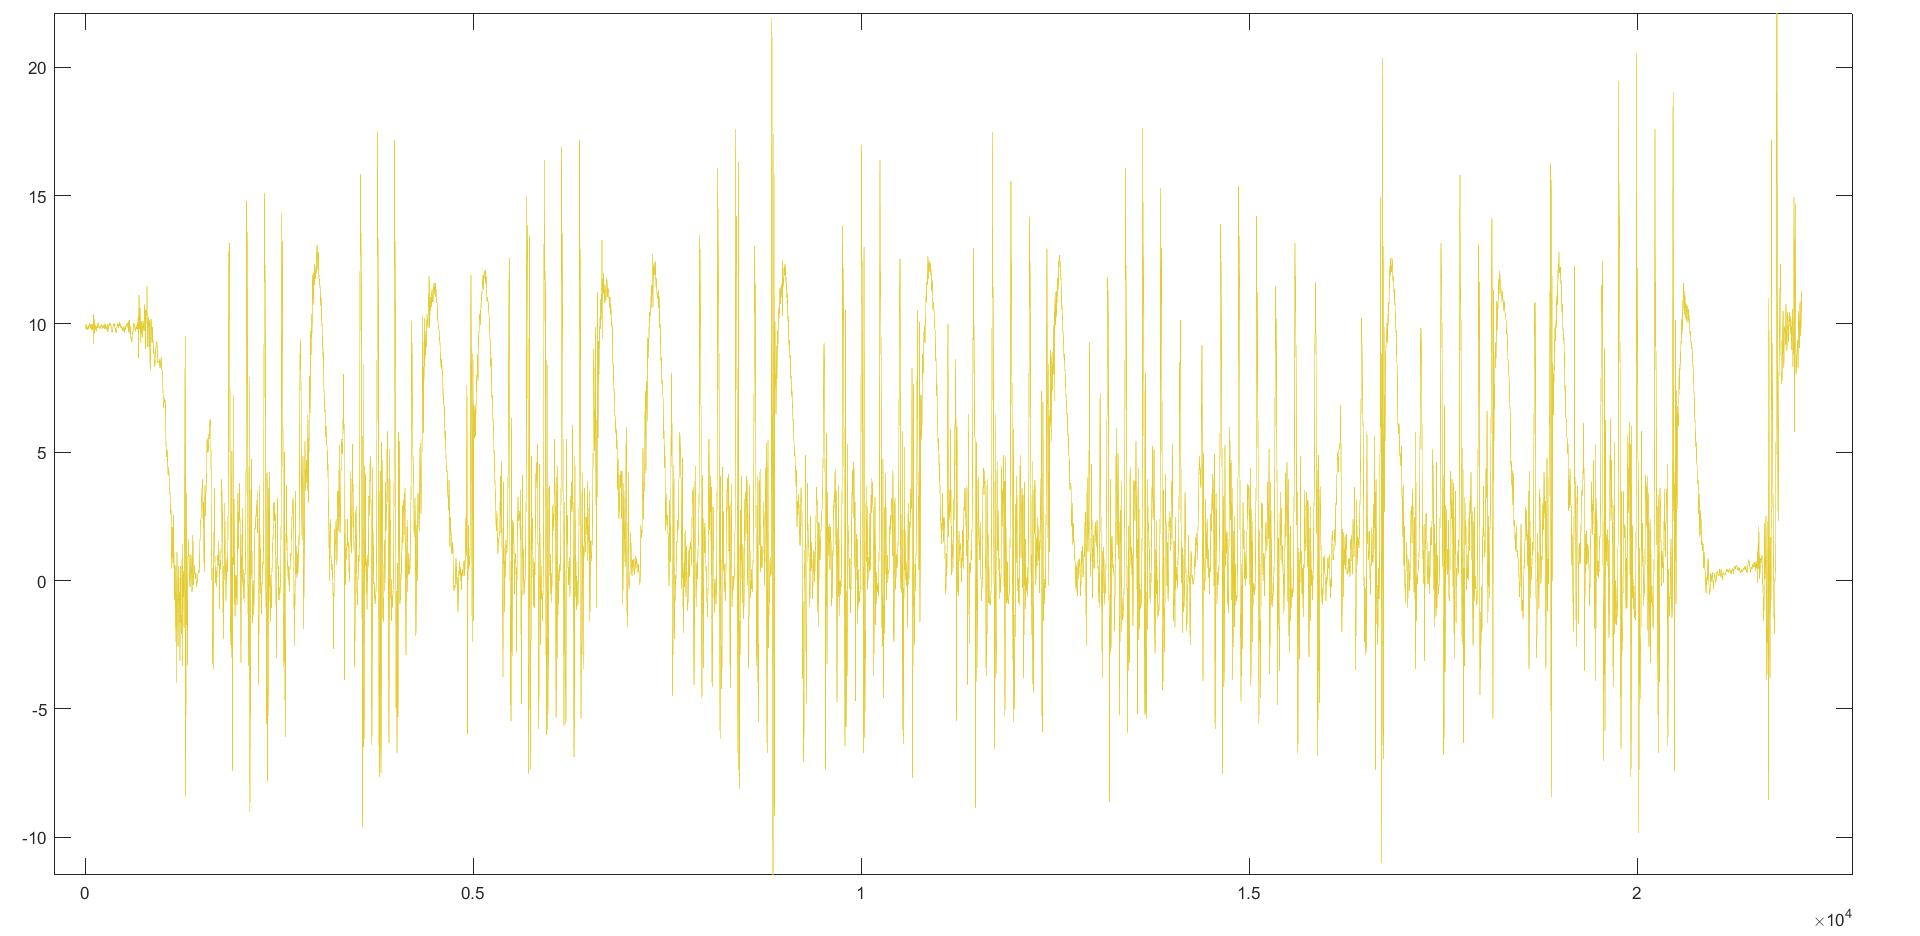
\includegraphics[width=154mm, height= 40mm]{./images/registrazione_tesi/acc_phZ.jpg} 
\captionof{figure}{Scomposizione del segnale accelerometrico triassiale in tre grafici.\\}
\end{center}
\end{minipage}
\makebox[\linewidth]{}



% ---- GRAFICI MAGNETOMETRO ------
\subsubsection{Magnetometro smartphone}
\begin{minipage}{\linewidth}
\begin{center}
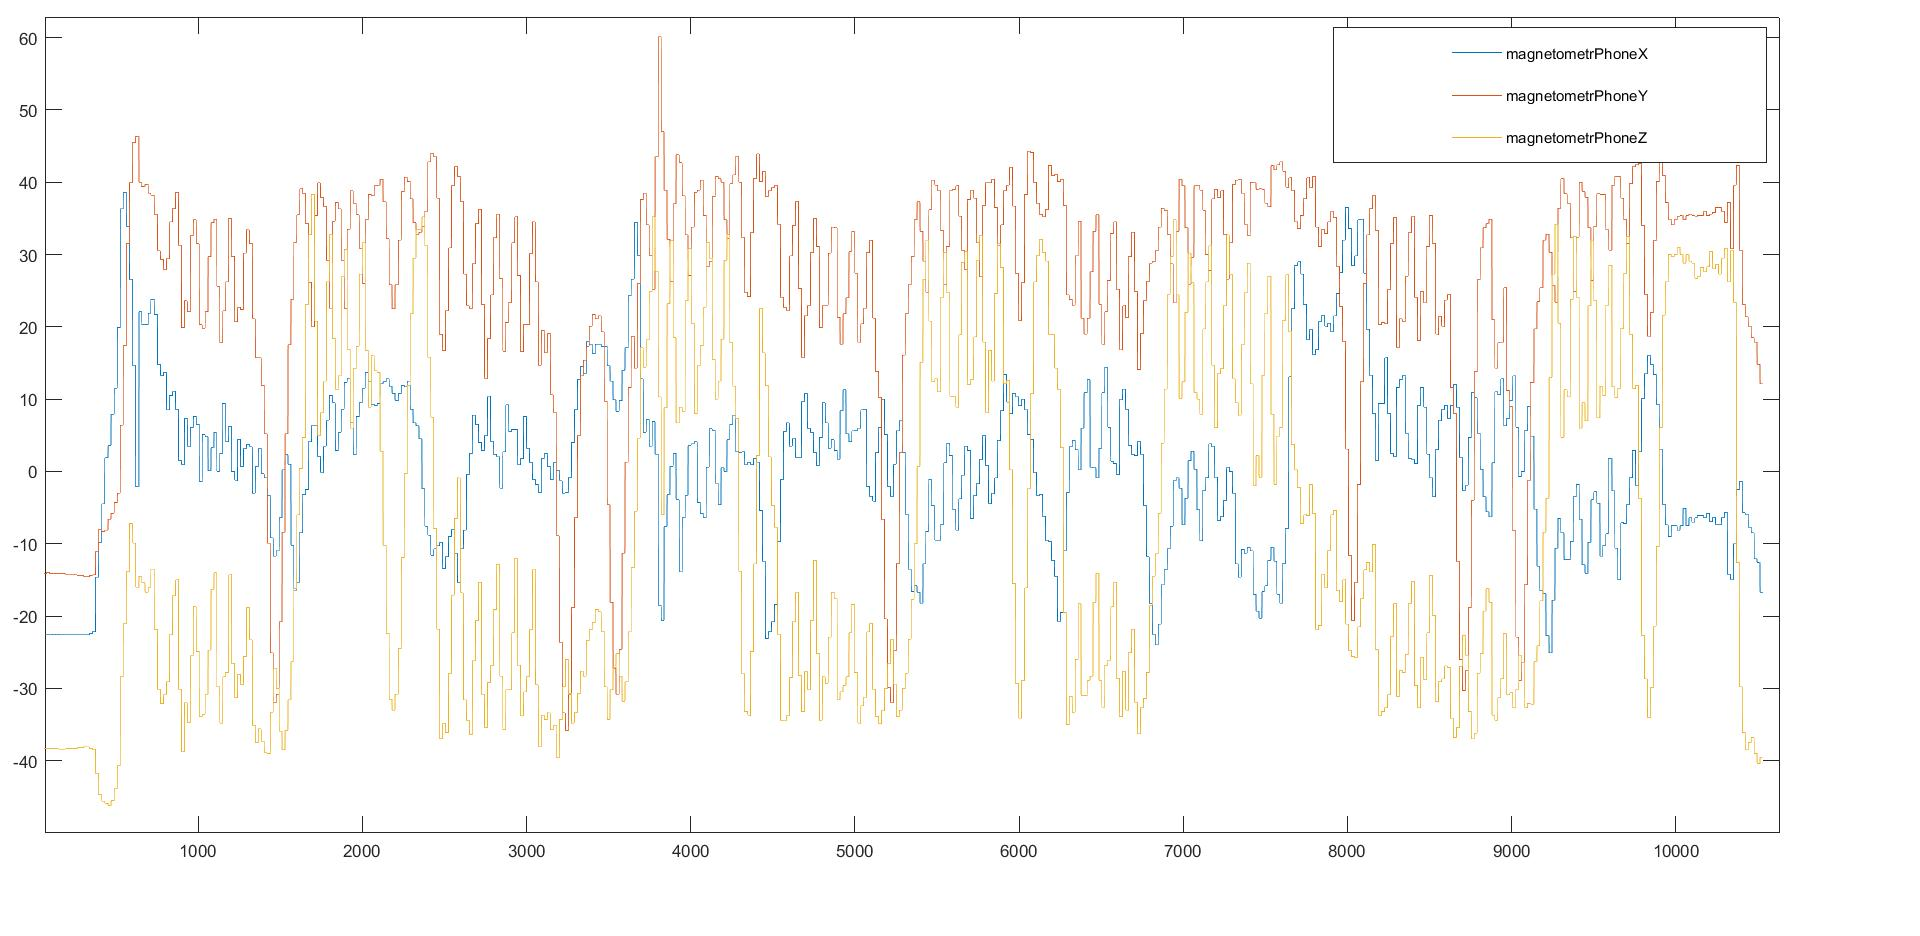
\includegraphics[width=160mm, height= 70mm]{./images/registrazione_tesi/mag_phXYZ.jpg} 
\captionof{figure}{Grafico accelerometro triassiale dello smartwatch.\\}
\end{center}
\end{minipage}
\makebox[\linewidth]{}
\makebox[\linewidth]{}\makebox[\linewidth]{}\makebox[\linewidth]{}
\makebox[\linewidth]{}\makebox[\linewidth]{}\makebox[\linewidth]{}
\makebox[\linewidth]{}\makebox[\linewidth]{}\makebox[\linewidth]{}

% ---- X -----
\begin{minipage}{\linewidth}
\begin{center}
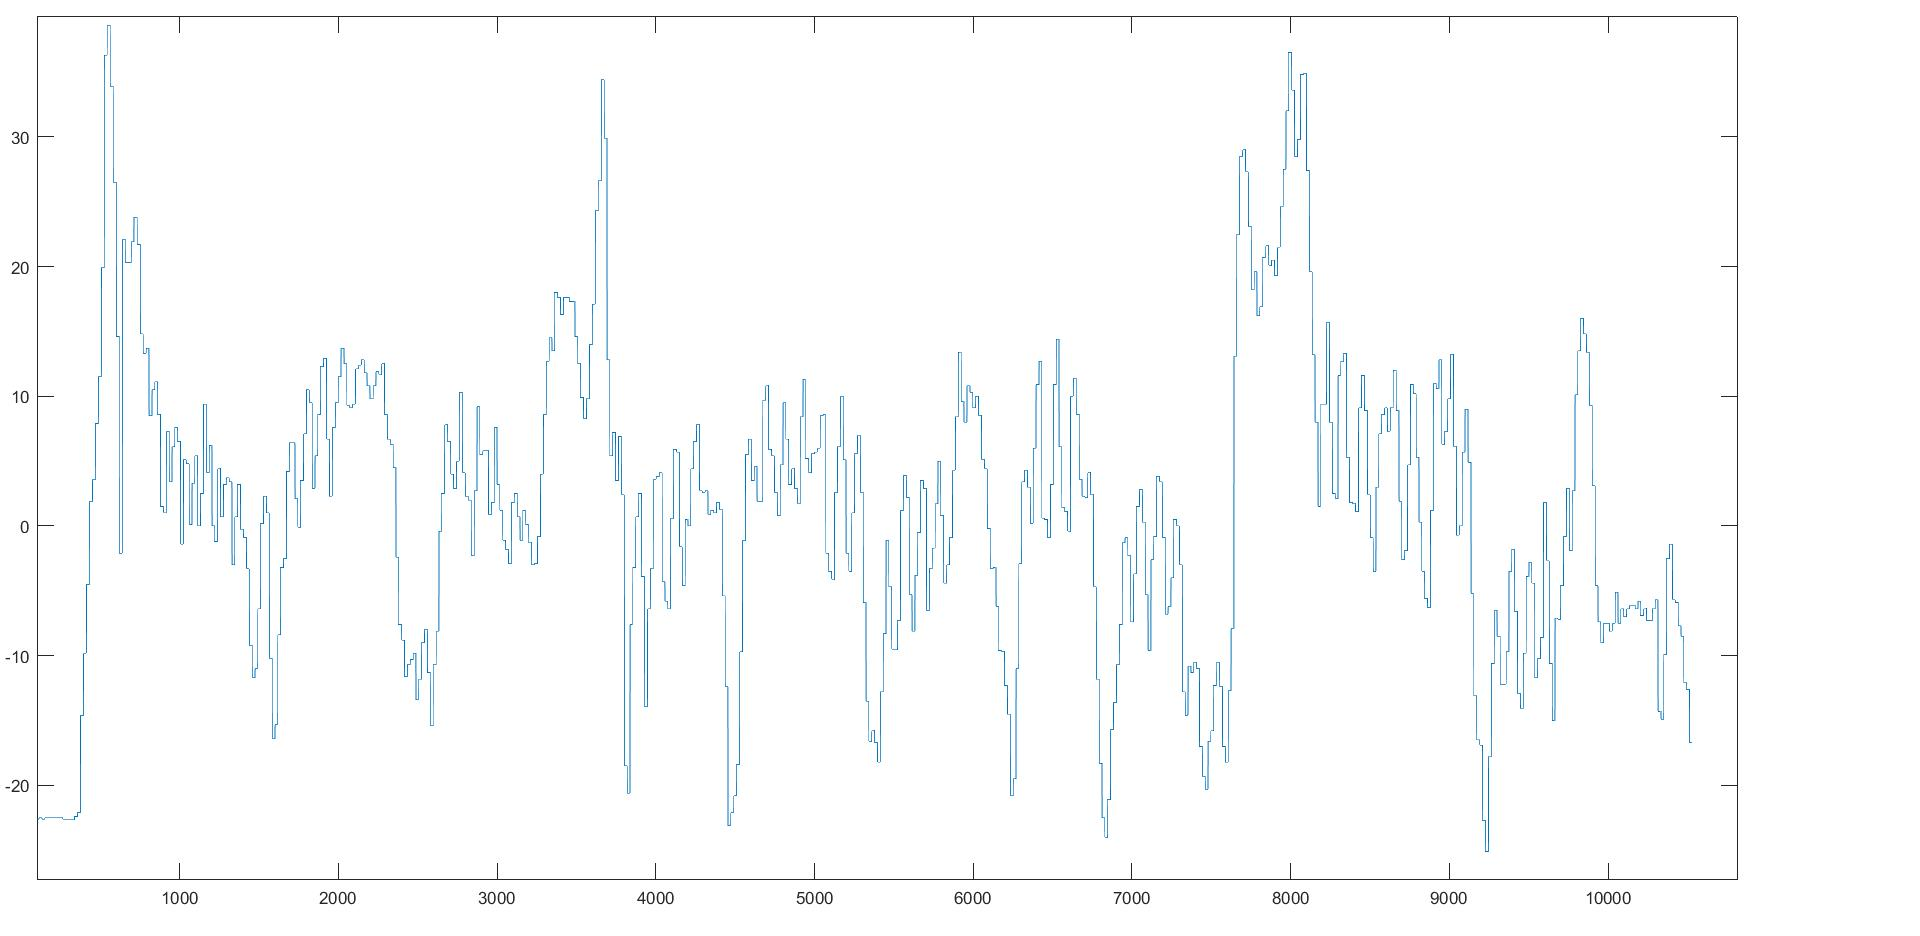
\includegraphics[width=154mm, height= 40mm]{./images/registrazione_tesi/mag_phX.jpg} 
\end{center}
\end{minipage}

% ---- Y -----
\begin{minipage}{\linewidth}
\begin{center}
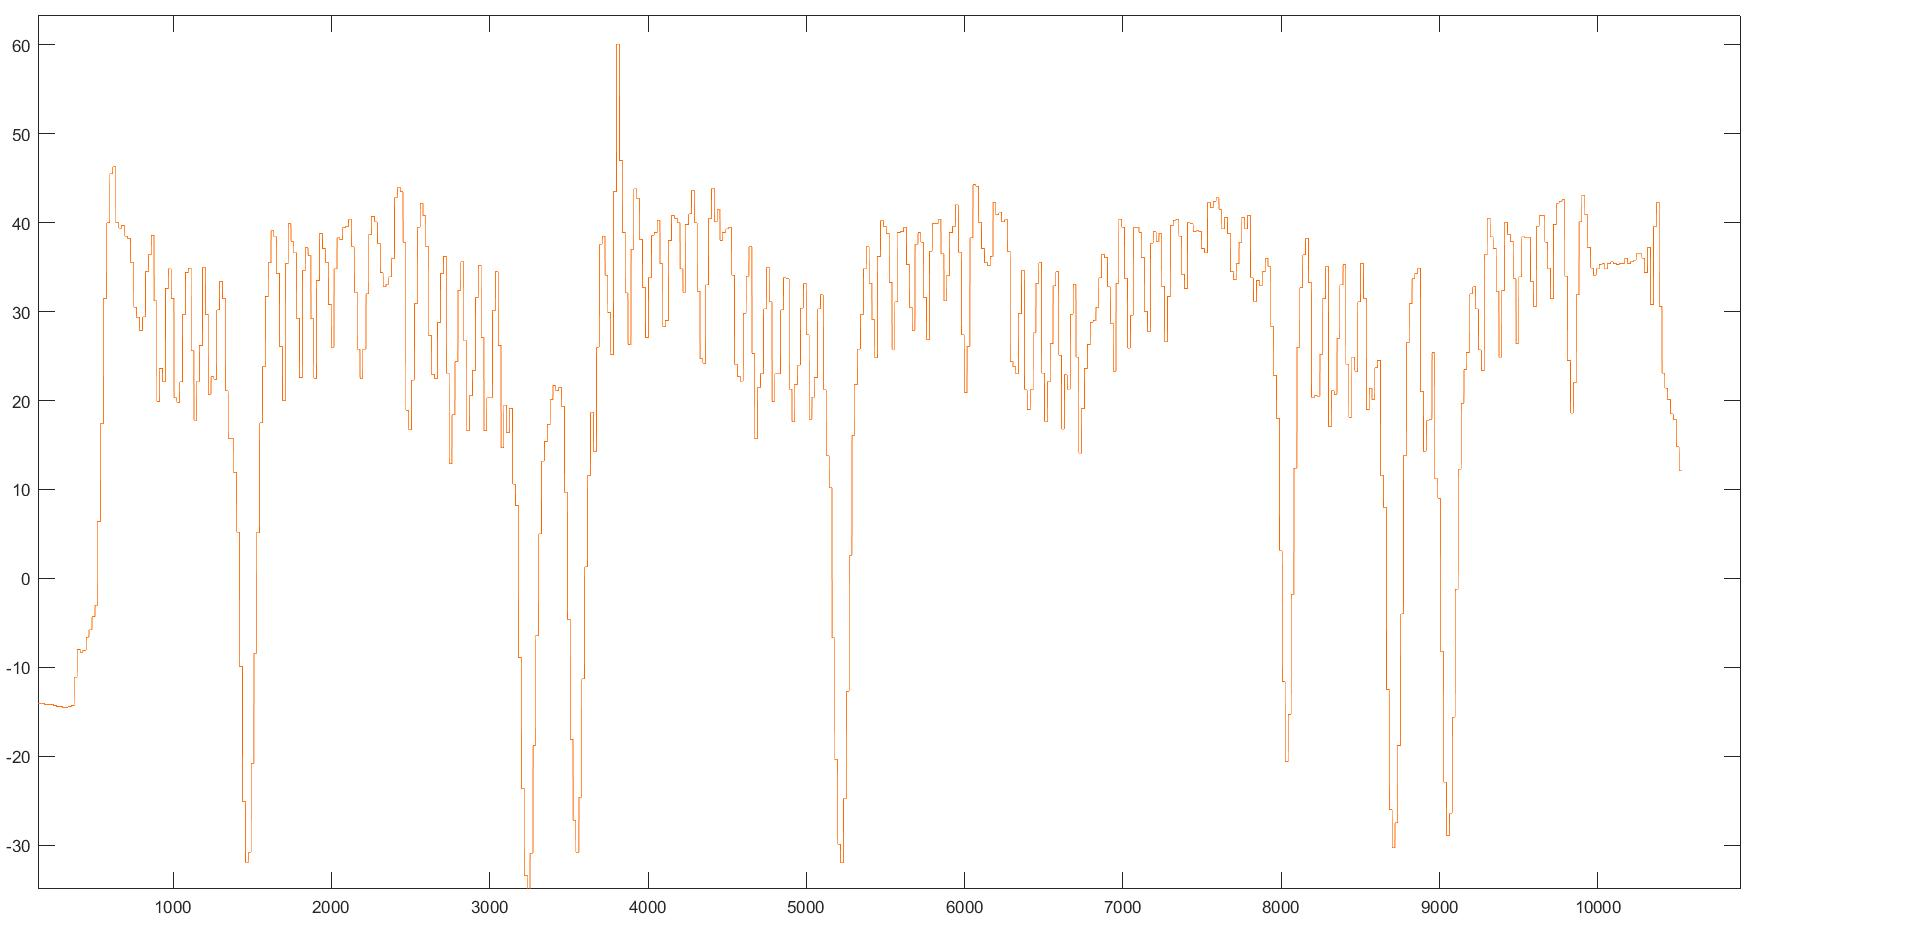
\includegraphics[width=154mm, height= 40mm]{./images/registrazione_tesi/mag_phY.jpg} 
\end{center}
\end{minipage}
\makebox[\linewidth]{}

% ---- Z -----
\begin{minipage}{\linewidth}
\begin{center}
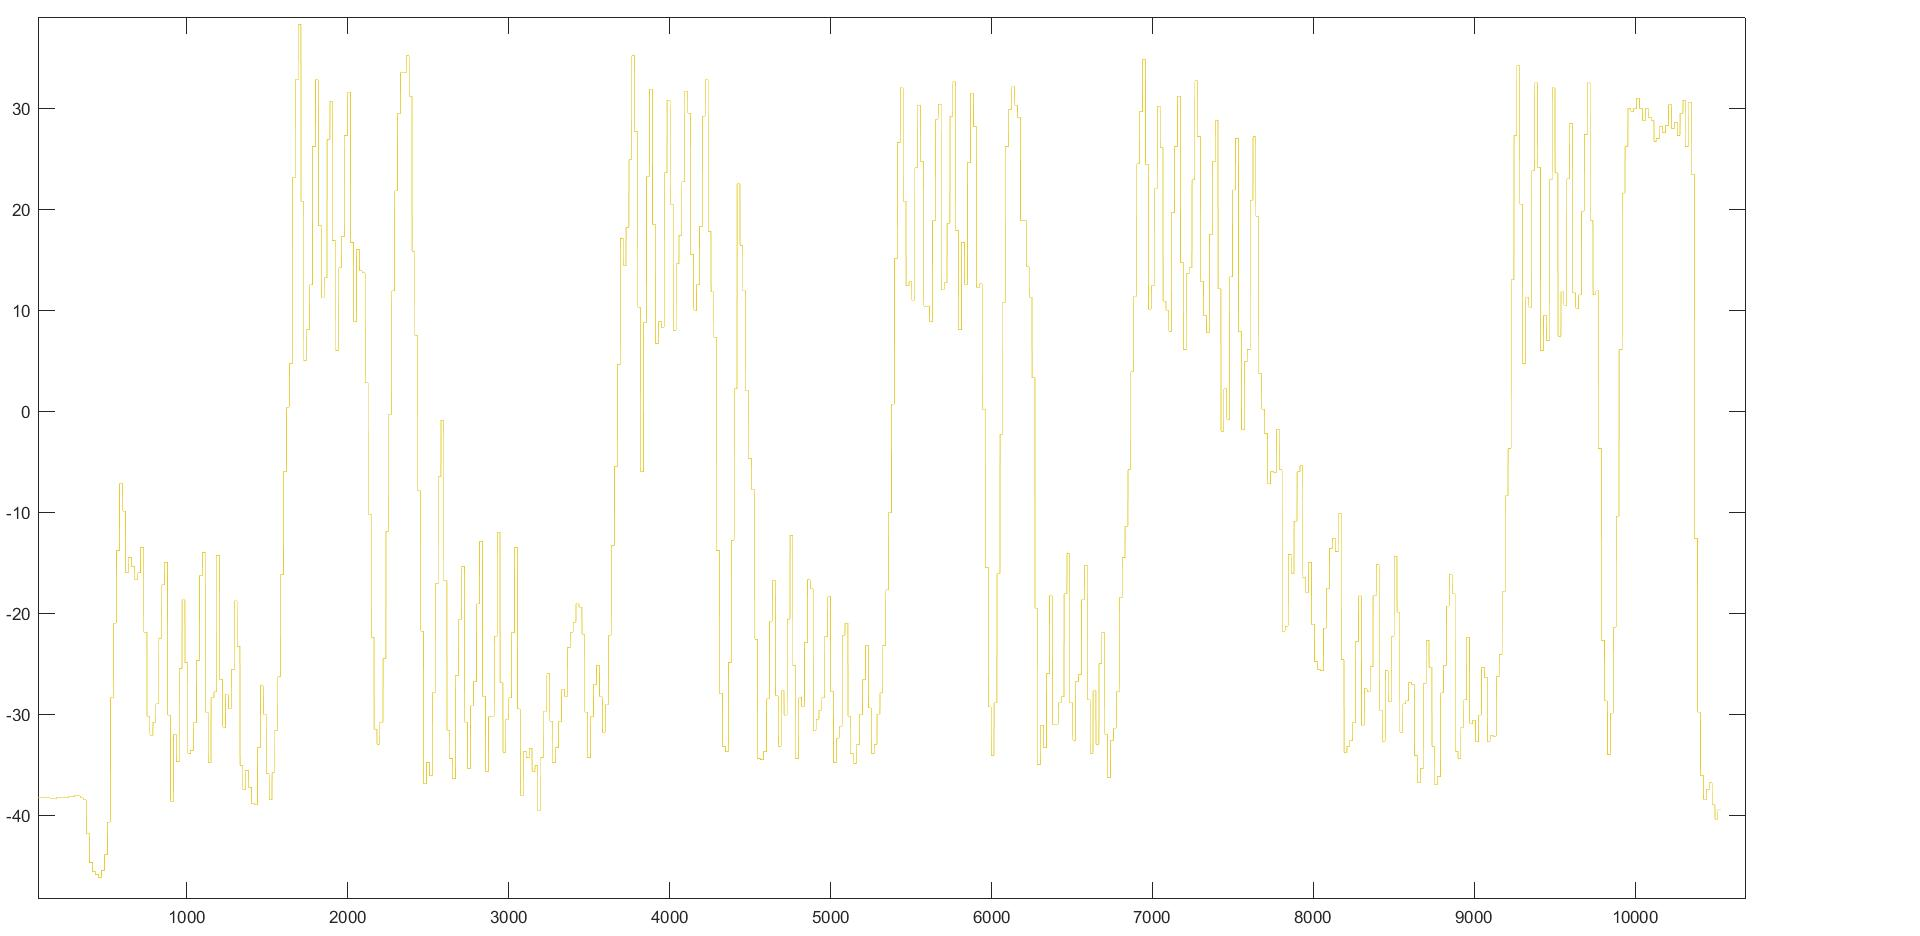
\includegraphics[width=154mm, height= 40mm]{./images/registrazione_tesi/mag_phZ.jpg} 
\captionof{figure}{Scomposizione del segnale magnetometrico triassiale in tre grafici.\\}
\end{center}
\end{minipage}
\makebox[\linewidth]{}


\clearpage

% ----- IL PROBLEMA DEGLI OUTLIER -----
\subsection{Il problema degli outlier}
Un problema che si riscontra dalla fase precedente, è la presenza di outlier: sample caratterizzati da valori non appartenenti ad un intervallo di valori attesi e numericamente distanti dal resto dei dati raccolti.  \\
I valori anomali possono avere molte cause, essendo dovuti a comportamenti fraudolenti del sistema: un apparato hardware per eseguire misurazioni potrebbe aver subito un malfunzionamento transitorio oppure potrebbe essersi verificato un errore nella trasmissione o trascrizione dei dati. \\
% , e che dovrà essere affrontato in fase di progetto e sviluppo
\begin{minipage}{\linewidth}
\begin{center}
\vspace{7mm}
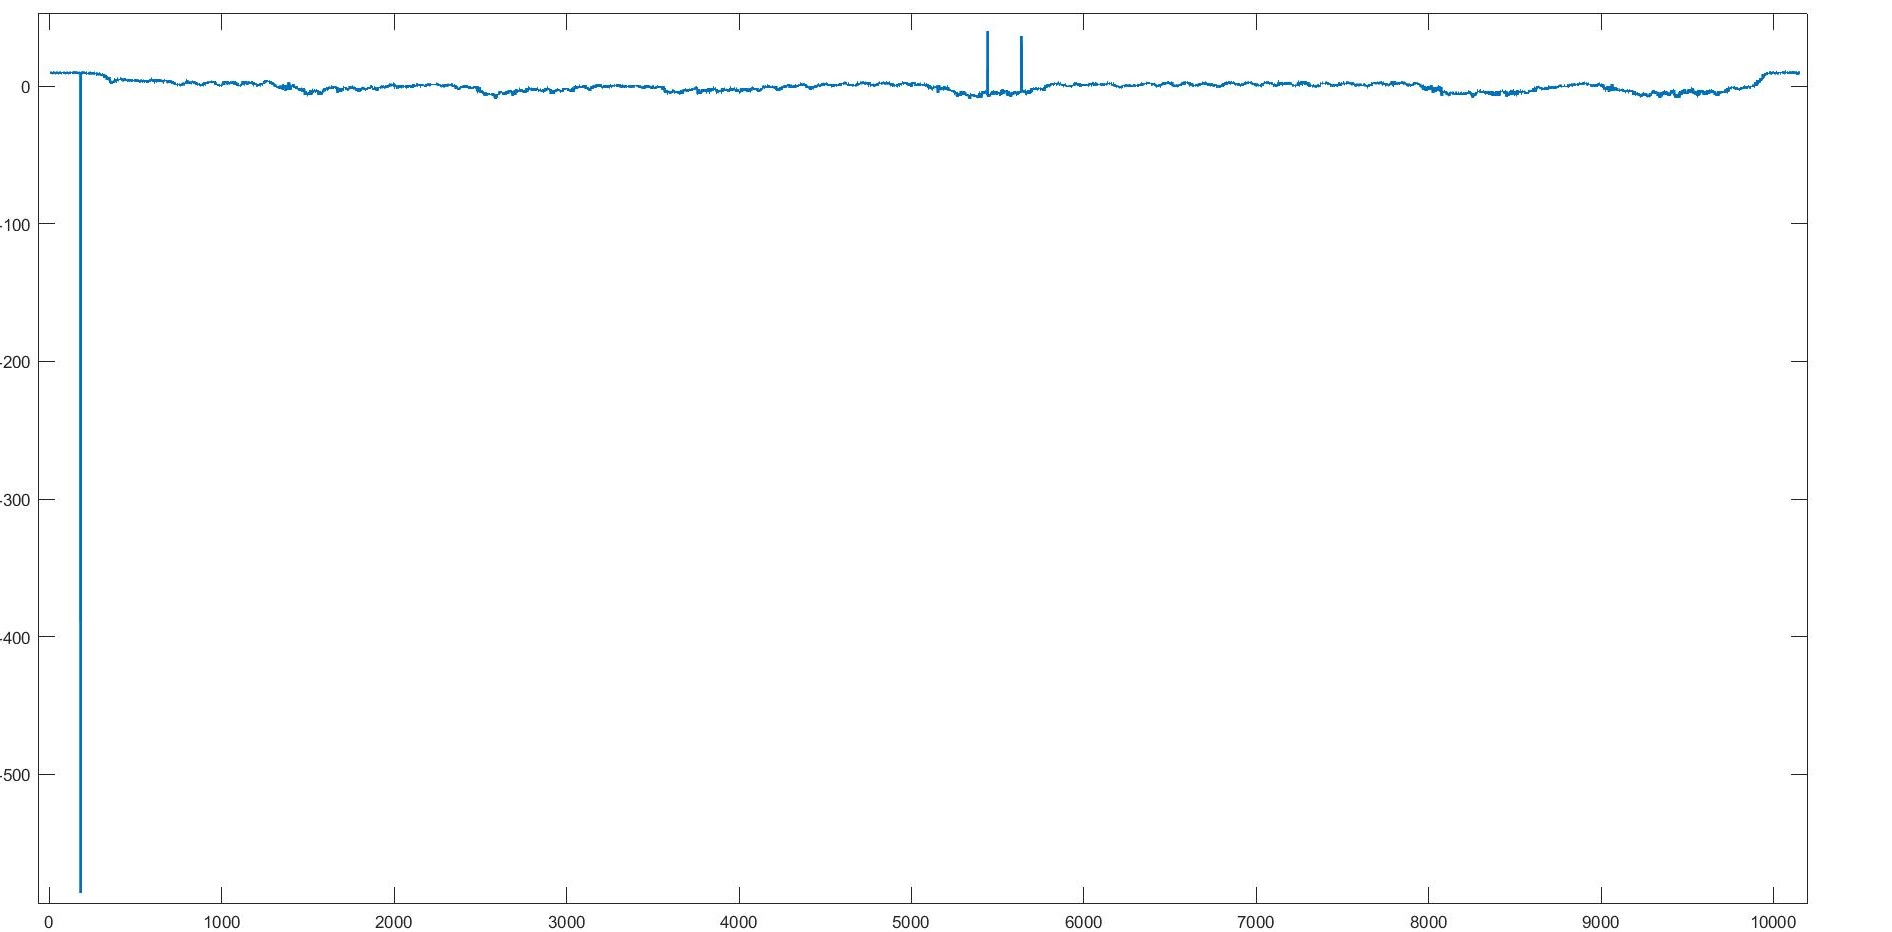
\includegraphics[width=154mm, height= 80mm]{./images/registrazione_tesi/outliers.jpg} 
\captionof{figure}{Grafico accelerometro asse X dello smartwatch.\\}
\vspace{7mm}
\end{center}
\end{minipage}
\makebox[\linewidth]{}
Costruendo il grafico dei segnali, è evidente la presenza di questi valori inattesi dai picchi che compaiono lungo il segnale, tali sample non permettono una scala ragionevolmente visualizzabile, per cui è neccessaria una fase di signal preprocessing, nella quale vengono eliminati questi campioni fuoriscala. \\
Essendo gli outlier un numero irrisorio (3 sample per il grafico in figura 15), possiamo procedere ad una pulizia manuale del segnale, cercando dal grafico generato da matlab, gli indici corrispondenti ai campioni presi in esame ed in seguito eliminarli.

% ----- ANALISI SEGNALE BAROMETRICO -----
\subsection{Il segnale barometrico per rilevare la manovra}


Il sensore che dà maggiori informazioni sul momento in cui avviene l’abbassamento è il barometro dell'orologio; nel grafico, infatti, si nota che in corrispondenza di un abbassamento si ha un innalzamento della pressione atmosferica del barometro, con un conseguente abbassamento quando ci si alza nuovamente.\\
L’elevato livello di rumore bianco di questo segnale rende difficile il compito di trovare delle regole generali per individuare algoritmicamente il momento in cui la persona si abbassa. \\
Inoltre, il sensore è affetto da disturbi che possono influenzare l’andamento del segnale (es. correnti d’aria o le variazioni di pressione generate dall’aprire o chiudere una finestra).
\makebox[\linewidth]{}
\makebox[\linewidth]{}
\begin{minipage}{\linewidth}
\begin{center}
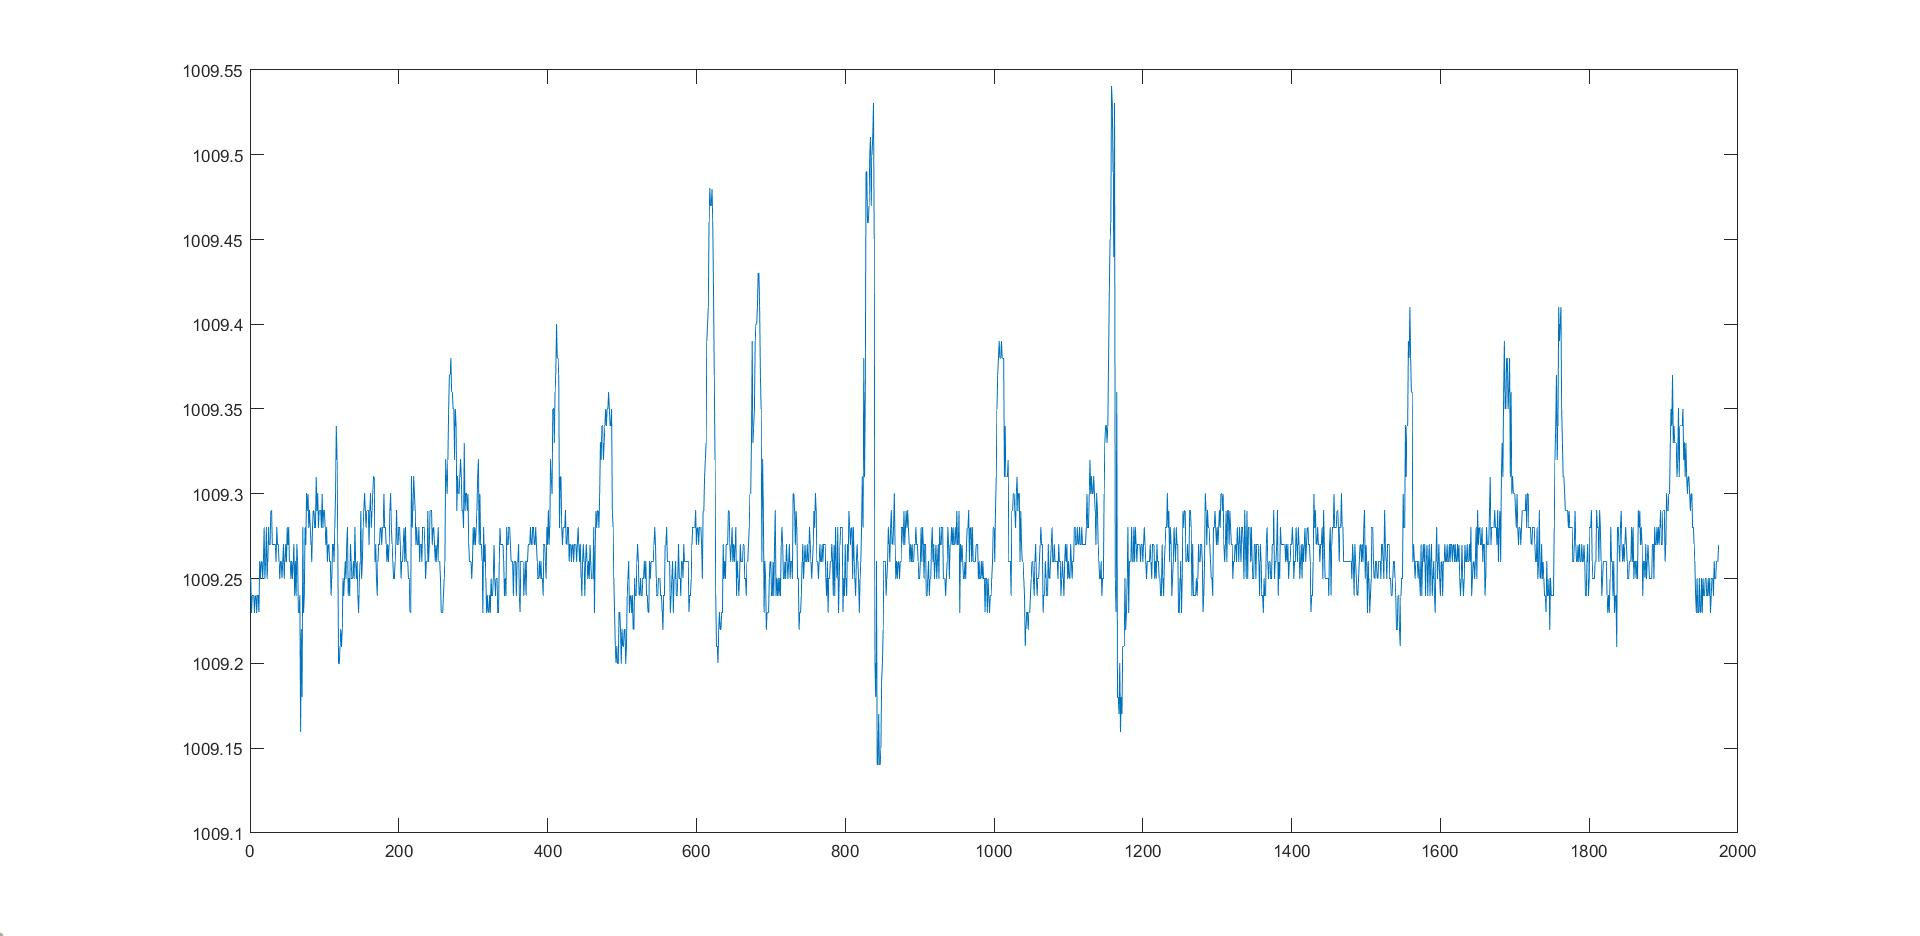
\includegraphics[width=150mm, height= 60mm]{./images/registrazione_tesi/pressure_watch.jpg} 
\captionof{figure}{Segnale barometrico dello smartphone.\\}
\end{center}
\end{minipage}
\makebox[\linewidth]{}
\makebox[\linewidth]{} 
%--
Per rendere più agevole la visualizzazione è opportuno applicare al segnale di partenza opportuni filtri. In particolare facendo vari tentativi, si giunge alla conclusione che, per ottenere una buonissima replica del segnale pulita e più lineare, si possono applicare un filtro a media mobile, seguito da un filtro gaussiano.
\begin {itemize}
\item Filtro a media mobile. Questo filtro prevede di ricostruire il segnale sostituendo al valore di ogni campione la media di campioni vicini. E’ una tecnica matematica utilizzata per smussare le fluttuazioni nel segnale. Si dice "mobile" perché il numero degli elementi considerati è fisso (finestra), ma l'intervallo di tempo avanza.
\item Filtro Gaussiano. Questo filtro viene applicato in cascata al precedente; anche in questo caso viene effettuata una media dei vicini, non aritmetica ma ponderata, in particolare ogni elemento verrà normalizzato, usando i coefficienti di una funzione gaussiana.
\end{itemize}
Il seguente codice Matlab applica al segnale di partenza i due filtri, producendo i grafici riportati in seguito: \\
% ----- filtri -----
\begin{lstlisting}[language=Matlab,  basicstyle=\footnotesize]
	watch_mov = movmean(pressurewatch(:,2),50);
	watchgaussian = smoothdata(watch_mov,'gaussian');
	plot(watch_mov);
	plot(watchgaussian)
\end{lstlisting}
\makebox[\linewidth]{}
\makebox[\linewidth]{}
\begin{minipage}{\linewidth}
\begin{center}
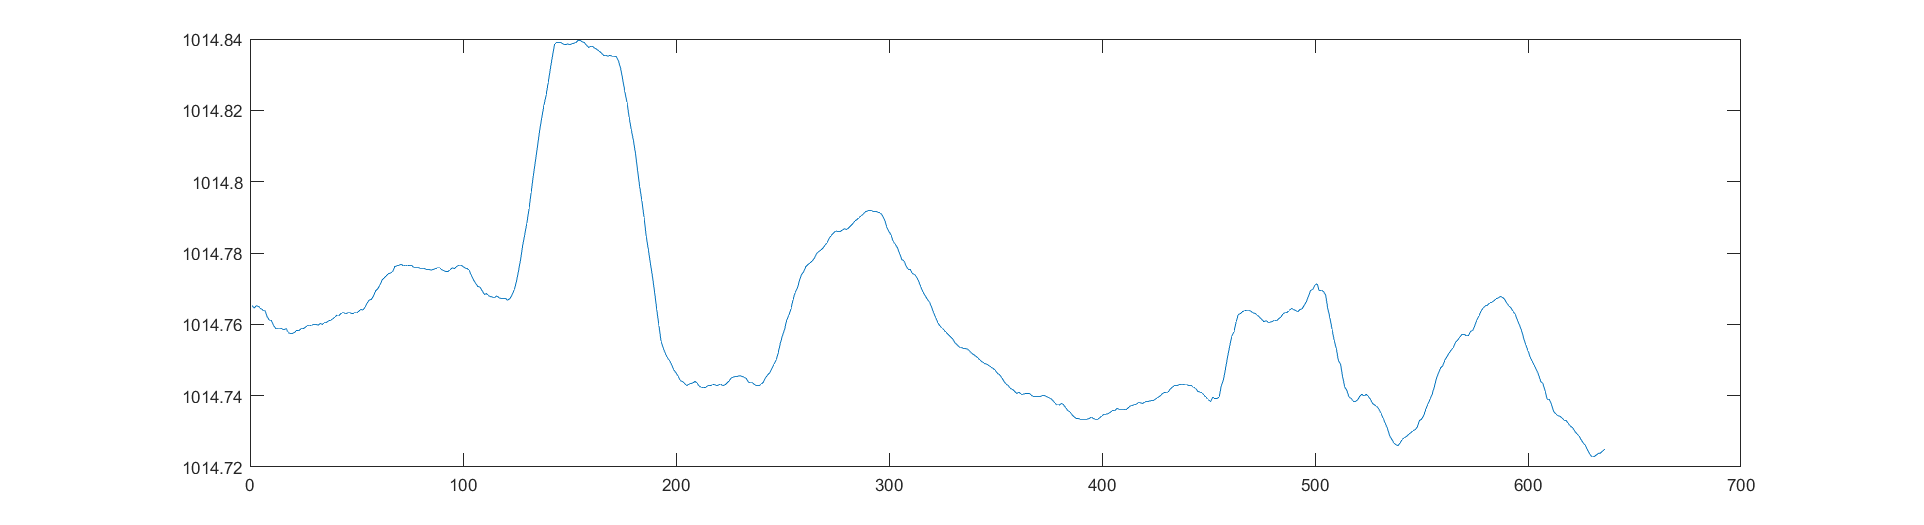
\includegraphics[width=160mm, height= 60mm]{./images/segnali/pressure_phone_movmean.png} 
\captionof{figure}{Segnale barometrico a cui è stato applicato il filtro a media mobile.\\}
\end{center}
\end{minipage}
\makebox[\linewidth]{}
\makebox[\linewidth]{}
\makebox[\linewidth]{}
\makebox[\linewidth]{}
\begin{minipage}{\linewidth}
\begin{center}
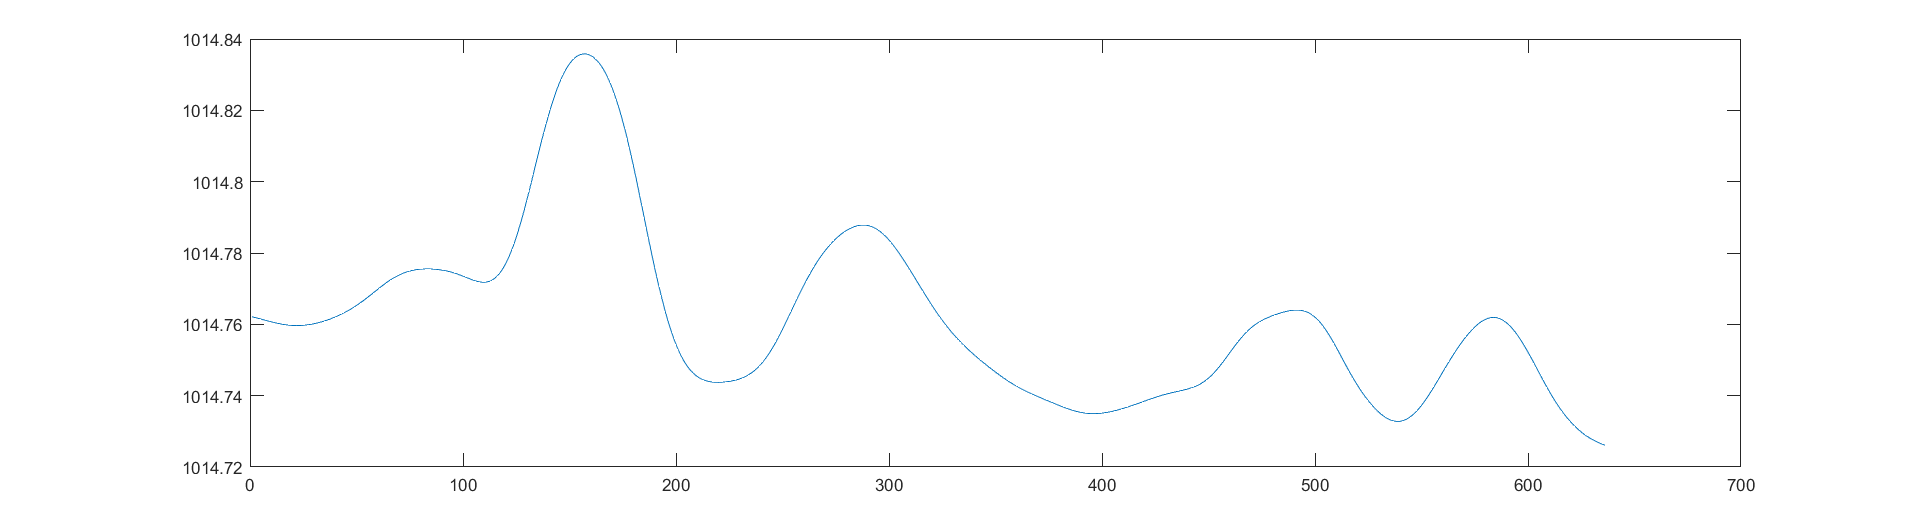
\includegraphics[width=160mm, height= 60mm]{./images/segnali/pressure_phone_gauss.png} 
\captionof{figure}{Segnale barometrico a cui sono stati applicati i filtri a media mobile e gaussiano.\\}
\end{center}
\end{minipage}



\clearpage

% ----- CAPITOLO V : Sviluppo applicazione realtime -----
\section{Sviluppo Applicazione Realtime}
Durante la fase finale è stato realizzato un sistema per il monitoraggio della movimentazione in tempo reale, seguendo i medesimi passaggi compiuti nella fase di analisi (vedi paragrafo 4). Infatti, anche questa fase, è divisa in due parti: l'individuazione degli istanti in cui sono state compiute le manovre, seguita dalla classificazione di queste ultime.\\
In realtà non è propriamente corretto definire questa applicazione realtime, in quanto la rilevazione non è immediata, ma si presenta un tempo di latenza dovuto principalmente all'aplicazione di filtri al segnale grezzo. Come spiegato nei paragrasfi successivi, al segnale registrato, vengono applicati due filtri a media mobile: in questo tipo di filtro si considera un certo numero di campioni N, detto FINESTRA, per calcolare il valore del segnale ad un determinato passo; dunque è neccessario aver collezionato gli N/2 campioni precedenti e gli N/2 successivi. Se considerando che vengono applicati due filtri di questa tipologia in cascata, sono neccessari un numero "elevato" di campioni futuri, per calcolare il valore del segnale ad un istante precedente.\\
Il sistema è implementato da un'applicazione Android, divisa in tre moduli, come l'applicazione utilizzata durante la fase della raccolta dei dati (vedi paragrafo 3.2): 
\begin {itemize}
\item \textbf{wear}, per la fase di detection
\item \textbf{mobile}, per la fase di classificazione.
\item \textbf{shared\_mobile\_watch}, una semplice libreria per la condivisioni di classi comuni ad entrambi i moduli precedenti \\
\end{itemize}


% ----- DESCRIZIONE MODULO WEAR E FUNZIONALITA' PRINCIPALI -----
\subsection{Detection}
La fase di detection degli istanti in cui è avvenuto il task del sollevamento è sviluppato nel modulo \textit{wear}.
La fase di detection degli istanti in cui è avvenuto il task del sollevamento è sviluppato nel modulo wear, in quanto è il sengale che, se pulito correttamente dai rumori, è quello che evidenzia meglio il compimento di un abbassamento. 

% ----- OPZIONI SU COME REALIZZARE I FILTRI -----
\subsubsection{Realizzazione dei filtri per la pulizia del segnale}
Il primo passo compiere una scelta progettuale: come implementare i filtri per la pulizia del segnale, che realizzino il medesimo comportamento delle funzioni Matlab \textit{movmean(signal, window\_size)} e \textit{smoothdata(signal, 'gaussian')}, citate precedentemente (vedi paragrafo 4.1). Alcune opzioni possibili sono le seguienti: 
\begin{itemize}
\item {scrivere uno script matlab (.m) contenente una funzoine ed esportare un un file .cpp (o .c) generato da Matlab, contenente del codice scritto nel linguaggio di programmazione C++ (oppure C), da includere nel progetto Android ed utilizzare Android Native Kit (NDK), per sviluppare questa porzione del modulo. \\
Questa opzione è molto valida, e dunque da prendere in considerazione per una versione più ottimizzata del sistema; in particolare perchè l'utilizzo del linguaggio C/C++ su Andoroid, viene fatto nei casi in cui si presentino probemi di calcolo computazionale, che appunto sono risolti con questa tecnica. 
Tuttavia non è stata fatta presa come scelta, a causa delle complicazioni che introduce nello sviluppo del progetto.\\
Il seguente script matlab mostra la funzione da scrivere, che prende come argomento un array di valori (il segnale grezzo) e e come tipo di ritorno restituisce un altro array di valori (il segnale filtrato).\\
% ----- funnzione per il filtraggio -----
\begin{lstlisting}[language=Matlab,  basicstyle=\footnotesize]
function gaussian_signal = signal_filter(x)
    watch_mov = movmean(x,50);
    gaussian_signal = smoothdata(watch_mov,'gaussian');
end
\end{lstlisting}}
\item{facendo riferimento allo script matlab del punto precedente, è possibile creare un Package java, grazie al tool \textbf{MATLAB Builder JA}; includendo il file .jar prodotto all'interno del progetto android, è possibile effettuare la pulizia del segnale. \\
Questa progedura ha come inconveniente la generazione di codice ridondante, per cui la scelta presa è quella descritta nel seguente punto.}
\item{implementare from scratch i due filtri necessari. L'implementazione sarà descritta nel seguente paragrafo.}
\end{itemize}

% ----- VALUTAZIONE DIMENSIONI BUFFER E INTRODUZIONI VARIABILI -----
\subsubsection{Memorizzazione dei segnali e valutazione delle lunghezze dei buffer}
Il secondo passo da compiere, per realizzare questo modulo, è lo storage dei campioni che descrivono un certo segnale. Non potendo mantere in memoria tutto il segnale registrato dal barometro, perchè potenzialmente infinito, è molto importante definire la quantità di campioni che possiamo memorizzare, per questioni legate principalmente alle risorse limitate dei dispositivi di cui ci siamo dotati. \\
Per questa parte di modulo è necessario mantenere in memoria tre buffer, uno per il segnale grezzo \textit{noisy\_signal}, uno per il segnale a cui viene applicato il primo filtro \textit{movmean\_signal} e l'ultimo per il segnale pulito finale \textit{gaussian\_signal}. In particolare la scelta che è stata fatta è di 50 campioni per il primo segnale, poichè la frequenza di campionamento è di 50 Hz, e di 100 campioni per quanto riguarda i secondi due segnali, poichè dalla fase di analisi si può notare che il compimento di un abbassamento, corrisponde a circa 100 campioni del segnale barometrico dello smartwatch. Questi variabili costanti possono essere soggette a modifiche, in quanto valutate euristicamente, in particolare la dimensione dei secondi due buffer; dunque compiendo uno studio in futuro più dettagliato sulle modalità e i tempi, con cui può essere compiuto questo task, si possono modificare queste dimensioni, in modo da migliorare i risultati. \\
% -----variabili per il progetto realtime -----
\begin{lstlisting}[language=Java,  basicstyle=\footnotesize]
 	private static int WINDOW_SIZE = 50;
	private static int GAUSSIAN_WINDOW_SIZE = 100;
	private static int PORTION_OF_SIGNAL = 100;

	ArrayList<Float> noisy_signal;	
	ArrayList<Float> movmean_signal;
	ArrayList<Float> gaussian_signal;
\end{lstlisting} 
\vspace{3mm}
Ioltre per ognuno dei precedenti segnali, viene memorizzato un array della stessa dimensione, per i timestamp: stesso indice descrive valore e istante di tempo dello stesso campione: \textit{ArrayList<Long> noisy\_signal\_timestamp; ArrayList<Long> movmean\_signal\_timestamp; ArrayList<Long> gaussian\_signal\_timestamp;}

% ----- IMPLEMENTAZIONE FILTRI ------
\subsubsection{Implementazione filtri}
\vspace{2mm}
% -----variabili per il progetto realtime -----
\begin{lstlisting}[language=Java,  basicstyle=\footnotesize]
  if(event.sensor.getType() == 6){ // PRESSURE

    noisy_signal.add(event.values[0]);
    noisy_signal_timestamp.add(event.timestamp);
    counter++;

    if(counter == WINDOW_SIZE){
        for(Float f : noisy_signal)
            media += f;
        media /= WINDOW_SIZE;
    }

    if(counter > WINDOW_SIZE){

        Float removed = noisy_signal.remove(0);
        noisy_signal_timestamp.remove(0);
        media = media + ((event.values[0] - removed) / WINDOW_SIZE);

        movmean_signal.add(media);
        movmean_signal_timestamp.add(noisy_signal_timestamp.get(WINDOW_SIZE/2));

        if(counter >  GAUSSIAN_WINDOW_SIZE + WINDOW_SIZE){
            movmean_signal.remove(0);
            movmean_signal_timestamp.remove(0);

            Float fl = gaussian_average(movmean_signal);


            gaussian_signal.add(fl);
            gaussian_signal_timestamp.add(movmean_signal_timestamp.get...
					...(GAUSSIAN_WINDOW_SIZE / 2));

            if(counter >  WINDOW_SIZE + GAUSSIAN_WINDOW_SIZE + PORTION_OF_SIGNAL){
                gaussian_signal.remove(0);
                gaussian_signal_timestamp.remove(0);
            }
        }
    }
}
\end{lstlisting}
\vspace{5mm}

% ----- TESTING MODULO DETECTION -> il fallimento :'D ------
\subsubsection{Testing modulo detection}
In questa fase è emersa l'impossibilità di poter realizzare il modulo di rilevazione della manovra, come descritto nel paragrafo 5.1.2, poichè l'applicazione di 3 filtri in cascata è un'oprazione di complessità, sia temporale che spaziale, non indifferente, per cui l'orologio non riesce a stare al passo del calcolo del segnale filtrato con l'arrivo dei campioni dai vari sensori. In particolare eseguendo l'applicazione in modalità debug e andando a leggere lo stacktrace, si può notare come l'esecuzione del Garbage-Collector (un thread Daemon che sta in esecuzione in background, che si occupa della gestione della memoria) non permetta al Main-thread di mantere traccia dei campioni e di calcolarne il sengale pulito.

% ----- SECONDA IMPLEMENTAZIONE FILTRI ------
\subsubsection{Seconda implementazione filtri}
In questa parte dello sviluppo dell'applicazione si è reso necessario riprogettare il modulo della detection in modo che non sia computazionalmente pesante per smartwatch: lo smoothing del segnale viene fatto solamente con un filtro a media mobile. \\
La rilevazione del picco e dunque dell'abbassamento, invece, viene fatta eseguendo un'analisi dell'andamento del segnale filtrato: data una finestra si campioni, si divide quest'ultima in 10 sottofinstre e per ciascuna si calcola la media, dopo di che si verifica che i primi 5 valor medi abbiano un andamento crescente, metre i secondi 5 un andamento decrescente; la verifica di questa condizione implica la presenza di un abbassamento. In generale questo approccio per la verifica dell'abbassamento, è sviluppato sulla falsa riga della media mobile, perchè stiamo descrivendo il segnale, mediante la media tra un sottinsime di campioni.
\vspace{2mm}
% ----- android mobile module -----
\begin{lstlisting}[language=Java,  basicstyle=\footnotesize]

    case 6:
        noisy_signal.addLast(event.values[0]);
        noisy_signal_timestamp.addLast(event.timestamp);
        counter++;


        if(counter == WINDOW_SIZE){
            for(Float f : noisy_signal)
                media += f;
            media /= WINDOW_SIZE;
        }

        if(counter > WINDOW_SIZE){

            Float removed = noisy_signal.removeFirst();
            noisy_signal_timestamp.removeFirst();
            media = media + ((event.values[0] - removed) / WINDOW_SIZE);

            movmean_signal.addLast(media);
            movmean_signal_timestamp.addLast(noisy_signal_timestamp.get
                                                        (WINDOW_SIZE/2));

            temp += media;
            if((counter \% FINDPEAK_WINDOW) == 0) {
                temp /= FINDPEAK_WINDOW;
                avg_array.addLast(temp);
                temp = 0.0f;
            }
            if(counter > MOVMEAN_WINDOW_SIZE + WINDOW_SIZE){
                movmean_signal.removeFirst();
                Long time = movmean_signal_timestamp.removeFirst();
                resize_windows(time);

                if((counter \% FINDPEAK_WINDOW) == 0)
                    avg_array.removeFirst();

                boolean peak = findPeak(avg_array);

                if(peak){
                    Log.i("PEAK", "TROOOOOOOOOOOOOOVATOOOOOOO");
                }
            }
        }
        break;
\end{lstlisting}
\vspace{2mm}
% ----- TESTING SECONDA IMPLEMENTAZIONE MODULO DETECTION ------
\subsubsection{Testing seconda implementazione modulo detection}
Durante la fase di testing della seconda implementazione si riscontra che il problema della scarsa potenza di calcolo dello smartwatch è risolto e che l'applicazione viene eseguita senza interruzioni o crash. \\
E' stato possibile, dunque, effettuare alcune simulazioni di abbasamento e raccolta di un oggetto da terra, per vedere se il sistema è in grado di comprendere se, chi indossa i dispositivi, ha effettivamente compiuto la manovra potenzialmente critica.\\
Dai risultati delle simulazioni, è emerso che il sistema realizzato è in grado di rilevare circa il 68\% degli abbasamenti. Ponendo attenzione agli abbassamenti non rilevati e interrogandosi sul motivo di questa mancanza, si nota che le manovre, di cui l'applicazione non è riuscita a fare la detection, sono quelle in cui l'utilizzatore è rimasto abbassato per più tempo, facendo durare la manovra più tempo: le manovre compiute in 2 sec / 2.5 sec. vengono indentificate, mentre gli abbasamenti compiuti in un tempo maggiore di 2.5 sec passano inosservati. \\
Per poter effettuare dei miglioramenti nei risultati ottenuti, sarebbe opportuno effettuare altre simulazioni, coinvolgendo più persone con differenti caratteristiche fisiche (altezza, età, sesso, ecc.), il cui obbiettivo è trovare la dimensione della finestra, e dunque il numero si sample, che megliono descrivono la manovra e grazie al quale viene minimizzato il numero di task non rilevati, così da poter cambiare il parametro constante \textit{static final int MOVMEAN\_WINDOW\_SIZE} ed ottenere un maggiore gradi di precisione.
\clearpage
% ----- CAPITOLO VI : conclusioni -----
	\section{Conclusione}


\clearpage
% ----- SITOGRAFIA -----
	\section{Sitografia}

\begin{itemize}
\item Documentazione Android, \textit{https://developer.android.com/docs}
\item Documentazione java Oracle, \textit{https://docs.oracle.com/en/java/index.html}
\item Documentazione Matlab, \textit{https://it.mathworks.com/}
\item Wikipedia, \textit{https://en.wikipedia.org/wiki/Main\_Page}
\end{itemize}




\end{document}


